\documentclass[12pt,onecolumn,a4paper]{book}

%% 引用宏包 %%
\usepackage{ctex}
\usepackage{titlesec}
\usepackage{amsmath,amssymb,amsthm,multicol,siunitx,graphicx,enumitem,booktabs,appendix}
\usepackage{booktabs}
\usepackage{tabularx,subcaption,arydshln}
\usepackage{tikz}
\usepackage{arydshln}
\usetikzlibrary{calc}
\usetikzlibrary{positioning}
\usepackage[edges]{forest}
\usepackage{pgfplots}

\usetikzlibrary{matrix, positioning, arrows}

\usepackage{imakeidx}
\usepackage{hyperref}

\makeindex

%% 定义新定理 %%
\newtheorem*{example}{例}
\newtheorem*{note}{注}

%% 设置初始编号 %%
\setcounter{section}{0}
\numberwithin{table}{subsection}
\numberwithin{equation}{subsection}

%% 设置超链接 %%
\hypersetup{
    hidelinks, % 取消红框
    colorlinks=true,
    linkcolor=blue,
    citecolor=black
}

%% BibTeX %%
\bibliographystyle{plain}
% \bibliography{}

%% 标题 %%
\title{逻辑学概论}
\author{AnZrew}
\date{癸卯春夏于清华园}

% \makeindex 
%%%%%%%%% 正文 %%%%%%%%%
\begin{document}

%% 制作标题 %%
\maketitle

\pagenumbering{roman}
\setcounter{page}{1}

\begin{center}
    \Huge\textbf{前言}
\end{center}~\

此笔记是根据2023春陈为蓬老师《逻辑学概论》的课堂与讲义整理而成。其中也有部分(尤其是注释部分)参考了网络资源如Wikipedia和ChatGPT整理得到。

逻辑学概论的课程介绍:

\begin{quotation}
    逻辑学是以有效推理形式为主要对象的工具性学科。逻辑学从古希腊和我国先秦以来,有着悠久的历史,逻辑学的现代形式是数理逻辑。本课程兼顾现代数理逻辑和传统形式逻辑,以数理逻辑的思路为纲,吸取传统逻辑中对日常推理有用的部分。内容涉及逻辑学的基础知识,包括命题、词项、推理、演绎、归纳、论证等,并简要介绍逻辑学发展史和现代逻辑发展情况,同时结合实际分析同逻辑有关的语言问题、同逻辑学有关的哲学问题。
\end{quotation}

此册用 \LaTeX 整理,内含超链接:文中蓝色字体均可点击跳转。

由于课程安排内容,章节前注有(*)非笔者所读学期重点掌握内容。

下面是笔者对于该课程的一个梳理,有助于从宏观上理解该课程的框架:

\newpage

\begin{forest}
    for tree={align=center,edge={->,>=latex}}
    [
        [逻辑\ref{chap1}
            [演绎逻辑系统
                [命题
                    [复合命题\ref{chap2}
                        [有效推理形式(范式\ref{chap3})\ref{chap2}]
                        [命题演算系统\ref{chap4}]
                    ]
                    [基本命题(词项)\ref{chap5}
                        [性质命题\ref{chap6},alias=prop]
                        [关系命题\ref{chap7},alias=rel]
                    ]
                ]
                [非标准逻辑\ref{chap9}]
            ]
            [归纳逻辑系统\ref{chap10}]
        ]
    ]
    \node[below=2cm] at (prop -| rel) (PredicateCalculus) {谓词演算系统\ref{chap8}};
    \draw[->] (prop) to[out=135,in=225] (PredicateCalculus);
    \draw[->] (rel) to[out=45,in=-45] (PredicateCalculus);
\end{forest}

图中后面的数字对应该文档里的章节。

祝学习愉快!

~\\
\begin{flushright}
    \begin{tabular}{c}
        AnZrew\\
        2023年夏
    \end{tabular}
\end{flushright}



\newpage
\pagenumbering{Roman}
\setcounter{page}{1}
\tableofcontents
\newpage
\setcounter{page}{1}
\pagenumbering{arabic}



\chapter{绪论:什么是逻辑}\label{chap1}

\section{逻辑[logic]}

\textbf{逻辑}\index{逻辑}一般指:

\begin{enumerate}[itemsep=0pt,parsep=0pt]
    \item 世界的可理解的规律
    \item 一般的原理和规则
    \item 语言、命题、说明、解释、论证
\end{enumerate}

而逻辑学是:研究推理的学科。

\section{逻辑学的研究对象:推理形式}

\textbf{推理:}\index{推理}从已知条件(前提)得到结论的过程。

\textbf{推理形式:}\index{推理形式}推理的结构。

同类的不同具体推理具有共同的结构,即推理形式。

\begin{table}
    \centering
    \begin{tabular}{c|c}
        所有M都是P & 所有M都是P \\
        S是M & S是P \\
        \hline
        S是P & S不是M \\
    \end{tabular}
\end{table}

\textbf{有效推理形式:}\index{有效推理形式}前提通过有效推理形式,只能得到真结论。这意味着结论假只可能是条件假。

\section{逻辑学的特点与基本准则}

\textbf{逻辑学的特点:}

\begin{enumerate}[itemsep=0pt,parsep=0pt]
    \item 抽象性:“甚至比数学的抽象性还要高”
    \item 应用性
    \item 工具性:需要和“材料”结合才有意义
\end{enumerate}

\textbf{逻辑学的基本准则:}

\begin{enumerate}[itemsep=0pt,parsep=0pt]
    \item 同一律:\index{同一律}A是A
    \item 矛盾律:\index{矛盾律}A不是非A A不能既是B又不是B
    \item 排中律:\index{排中律}A是B或A不是B必居其一
\end{enumerate}

\begin{example}
    哲学家大战逻辑学家:

    \begin{quotation}
        “有些事情既是好事又不是好事”
    \end{quotation}

    但事实上,这是面对不同方面的,这不与矛盾律相违背,即“既是B又不是C”。
\end{example}

\section{逻辑学的产生和发展}

\subsection{先秦中国古代逻辑思想}

\begin{enumerate}[itemsep=0pt,parsep=0pt]
    \item 孔子:正名
    \item 公孙龙:白马非马
    \item 语庄子:濠梁之辩
    \item 韩非子:矛盾之说
    \item 墨家逻辑思想
\end{enumerate}

\textbf{正名}【连锁推理】

\begin{quotation}
    \emph{名不正则言不顺,言不顺则事不成,事不成则礼乐不兴。(《论语》)}
\end{quotation}

\textbf{白马非马}【诡辩,集合论】

\begin{quotation}
    \emph{马者所以命形也,白者所以命色也。命色者非命形也,故曰白马非马。}

    \emph{求马,黄、黑马皆可致。求白马,黄、黑马不可致。 (《白马论》)}
\end{quotation}

问题出在“是”:“是”可以指$=$, $\in$, $\subseteq$。白马非马正是对“白$\neq$马”和“白马$\notin$马”的争论。

\textbf{濠梁之辩}【偷换概念,同一律、矛盾律】

\begin{quotation}
    \emph{子非鱼,安知鱼之乐?}

    \emph{子非我,安知我不知鱼之乐?}

    \emph{我非子,固不知子矣;子固非鱼也,子不知鱼之乐,全矣。}

    \emph{请循其本。子曰“如安知鱼之乐”云者,既已知吾知之而问我,我知之濠上也。 (《庄子·外篇·秋水》)}
\end{quotation}
问题出在“安”:“哪里”,表示地点,也表示否定。

采用了类比的方法。

这个辩论体现了庄子的智慧:“彼亦一是非,此亦一是非。”

\textbf{矛盾之说}【矛盾律】

\begin{quotation}
    \emph{以子之矛陷子之盾何如?不可陷之盾与无不陷之矛,不可同世而立。 (《韩非子·难一》)}
\end{quotation}
A与非A不能同时成立。

\textbf{墨家逻辑思想}后期墨家(墨子去世后)的《墨子·墨经》提出了比较完整的逻辑体系。

分为:《经上》《经下》《经说上》《经说下》《大取》《小取》,共六篇。

\begin{quotation}
    \emph{夫辩者,将以明是非之分,审治乱之纪,明同异之处,察名实之理,处利害,决嫌疑焉。}

    \emph{以名举实,以辞抒意,以说出故。 (《墨经·小取》)}
\end{quotation}
指出了辩论的重要性。

现代逻辑学中, 推理由命题 (判断) 组成, 命题由词项 (概念) 组成。上述话中,“名”、“辞”、“说”分别与“词项”、“命题”、“推理”相对应。

\subsection{印度佛学逻辑}

\textbf{因明}佛教中的推理理论。

玄奘在印度那烂陀的无遮大会以因明取胜,藏转佛教中也有辩经环节。

\subsection{古希腊逻辑}

\textbf{亚里士多德}(B.C.384-B.C.322)古希腊逻辑思想集大成者。

《亚里士多德全集》第一卷《工具论》:《范畴篇》《解释篇》《前分析篇》《后分析篇》《论辩篇》《辩谬篇》就奠基了理论基础,亚里士多德也透彻地分析了三段论理论。

\subsection{近代西方逻辑}

\textbf{弗兰西斯培根}(1561-1626)

《新工具》,提出了发现(归纳),思想(演绎),记忆,传递。强调了归纳的重要性,并提出了归纳的三表法——出现表(具有表)、不出现表(缺乏表)、程度表(比较表)。一般性的命题却是从大量经验所归纳的,对一般性命题的归纳比由其发出的演绎更重要。

\begin{example}
    p:“人固有一死”$\Rightarrow$q:“苏格拉底会死”

    看似是p推出q,事实上p本身是由诸多q的命题“归纳”得出的,是更原始性的命题。
\end{example}

\textbf{穆勒}(1806-1873)

归纳的求因果五法。

\subsection{数理逻辑的产生与发展}

\textbf{莱布尼兹}(1646-1716)

提出关于数学逻辑的思想,设想建立“普遍的符号语言”:思想的字母、思维的演算。

强调证明与统一的标准。

\textbf{布尔}布尔代数——一种命题演算

\textbf{罗素\&怀特海}(1872-1970)(1861-1947)

《数学原理》:建立完备的命题演算和谓词演算,从而完成逻辑演算。

\begin{note}
    命题演算:如果...那么... 谓词演算:全称/存在量词
\end{note}

\begin{note}[传统逻辑和数理逻辑]
    数理逻辑主要有以下:

    逻辑演算(命题演算、谓词演算)

    公理集合论、递归函数轮、证明论、模型论
\end{note}

\begin{note}[非经典逻辑]
    也称为非标准逻辑:

    经典逻辑(标准逻辑):二值,外延。

    非经典逻辑(非标准逻辑):多值逻辑(不全对、不全错),模糊逻辑,模态逻辑(可能、一定),广义模态逻辑,弗协调逻辑...
\end{note}

\section{逻辑学同其他学科关系}

\begin{itemize}[itemsep=0pt,parsep=0pt]
    \item 哲学:对语言进行逻辑分析,找到清楚而无歧义的论述方法。
    \item 数学:逻辑系统是数学的根基。
    \item 语言学
    \item 计算机科学
\end{itemize}

\section*{第一次作业}
\addcontentsline{toc}{section}{第一次作业} 

\begin{enumerate}[itemsep=0pt,parsep=0pt]
    \item 你选修《逻辑学概论》的初衷是什么?
    \item 此前你心中的“逻辑学”是什么样的?
\end{enumerate}

\chapter{复合命题的推理}\label{chap2}

\section{推理和命题}

\textbf{推理:}\index{推理}从前提(已知条件)得出结论的过程。

推理的前提和结论都是命题。

\textbf{命题(proposition或statement):}\index{命题}对事物及情况(性质、关系)的陈述。

命题只是完整的陈述,无关本身是否符合事实。

命题的\textbf{真值}\index{真值}:命题的真假情况。(二值逻辑与多值逻辑)

\emph{每一个命题都有真值,这是命题的基本性质。在经典逻辑中,真值取真/假两种情况。}

命题的真值是客观存在的,但真值为何可能是目前未有定论的。

\textbf{有效推理形式}\index{有效推理形式}若前提是真命题,那么通过有效推理形式所得到的只能是真命题。

若通过非有效的推理逻辑,有可能由真命题得到假命题。

\section{基本命题和复合命题}

\textbf{基本(简单)命题:}\index{基本命题}本身不包括其他命题的命题。

\textbf{复合命题:}\index{复合命题}由一个命题或多个基本命题加上命题联结词所构成的命题。(如果、那么、并非...)

\begin{example}
    以下是一些复合命题的例子:

    今天下大雪\emph{并且}今天刮大风。

    今天下大雪\emph{或者}今天刮大风。

    \emph{如果}今天刮大风,\emph{那么}明天会很冷。

    \emph{并非}今天下大雪。
\end{example}

\subsection*{基本命题和复合命题其真值的确定}

基本命题和复合命题有原则的区别:二者在真值的确定上有本质区别。即逻辑学上无法孤立判断基本命题的真值,但可以推测复合命题的真值。

\textbf{基本命题的真值:}逻辑学本身不涉及、不能确定的基本命题的真值。

\textbf{复合命题的真值:}由作为其组成部分的基本命题的真值和相关的命题联结词\index{命题联结词}的性质所决定。

某些有特定形式的复合命题,逻辑学本身即可确定真值。

\begin{example}
    这是可以判断真值的复合命题的例子:

    \begin{quotation}
    p或非p
    \end{quotation}

    这个命题一定是真的。
\end{example}

\emph{有趣的是,上述命题的真值的判断与逻辑学本身无关,是被认为的事实。(或属于元逻辑的范畴)}

\textbf{命题形式}\index{命题形式}即命题结构,用一定的符号表示。

\begin{example}
    以下是用符号表示的命题结构:
    \begin{equation}
    p\mbox{或非}p \Rightarrow p \wedge (\neg p)
    \end{equation}
\end{example}

\section{常用命题联结词极其基本推理形式}\index{命题联结词}\label{2.3}

\index{命题联结词}

\subsection{否定$\neg$}\index{否定}

\textbf{真值表:}\index{真值表}显示命题形式在各种可能下情况下的真值。

\emph{在真值表中,通常以$p_{1},p_{2},p_{3}$...或$p,q,r$...表示命题;以$T$表示真,$P$表示假。}

\begin{table}[h]
    \centering
    \setlength{\tabcolsep}{5mm}
    \begin{tabular}{cc}
        \toprule
        p & $\neg$p \\ 
        \midrule
        T & F\\
        F & T\\
        \bottomrule
    \end{tabular}
    \caption{否定的真值表}
\end{table}

基本推理形式:双重否定式

\begin{equation}
     p = \neg(\neg p)
\end{equation}

\textbf{【基本推理形式】}双重否定式

在逻辑学中,仅仅关于命题的真值,与强调“语气”无关。

\begin{equation}
     p = \neg(\neg p)
\end{equation}


\subsection{合取$\wedge$}\index{合取}

\begin{table}[h]
    \centering
    \setlength{\tabcolsep}{5mm}
    \begin{tabular}{ccc}
        \toprule
        p & q & p$\wedge$q \\ 
        \midrule
        T & T & T\\
        F & T & F\\
        T & F & F\\
        F & F & F\\
        \bottomrule
    \end{tabular}
    \caption{合取的真值表}
\end{table}

合取没有递进、转折的意味,仅仅表示并列关系。

\textbf{【基本推理形式】}

\begin{itemize}[itemsep=0pt,parsep=0pt]
    \item 构成式:已知p与q就可以合取
    \item 分解式
    \item 易位式:p,q地位是等价的
\end{itemize}

\begin{table}[h]
    \centering
    \begin{tabular}{ccc}
        \subcaptionbox{合取的构成式}[3cm]{
            \begin{tabular}{c}
                p\\ 
                q\\
                \midrule
                p$\wedge$q\\
            \end{tabular}
        }
        \hspace{1cm}
        &
        \subcaptionbox{合取的分解式}[3cm]{
            \begin{tabular}{c}
                p$\wedge$q\\ 
                \midrule
                p\\
            \end{tabular}
        }
        \hspace{1cm}
        &
        \subcaptionbox{合取的易位式}[3cm]{
            \begin{tabular}{c}
                p$\wedge$q\\
                \midrule
                q$\wedge$p\\
            \end{tabular}
        }
    \end{tabular}
    \caption{合取的构成式、分解式和易位式}
\end{table}


\subsection{析取$\vee$}\index{析取}

\begin{table}[h]
    \centering
    \setlength{\tabcolsep}{5mm}
    \begin{tabular}{ccc}
        \toprule
        p & q & p$\vee$q \\ 
        \midrule
        T & T & T\\
        F & T & T\\
        T & F & T\\
        F & F & F\\
        \bottomrule
    \end{tabular}
    \caption{析取的真值表}
\end{table}

\textbf{【基本推理形式】}

\begin{itemize}[itemsep=0pt,parsep=0pt]
    \item 构成式:已知p与q就可以析取
    \item 易位式
    \item 肯定否定式:析取关系中的一个部分为假,则另一部分为真
\end{itemize}

\begin{table}[h]
    \centering
    \begin{tabular}{ccc}
        \subcaptionbox{析取的构成式}[3cm]{
            \begin{tabular}{c}
                p\\ 
                \midrule
                p$\vee$q\\
            \end{tabular}
        }
        \hspace{1cm}
        &
        \subcaptionbox{析取的易位式}[3cm]{
            \begin{tabular}{c}
                p$\vee$q\\
                \midrule
                q$\vee$p\\
            \end{tabular}
        }
        \hspace{1cm}
        &
        \subcaptionbox{析取的肯定否定式}[5cm]{
            \begin{tabular}{c}
                p$\vee$q\\ 
                $\neg$ p\\
                \midrule
                q\\
            \end{tabular}
        }
    \end{tabular}
    \caption{析取的构成式、易位式和肯定否定式}
\end{table}

析取关系中,肯定一个不能代表否定另外一个。

\newpage

\subsection{不相容析取$\dot{\vee}$}\index{不相容析取}

\begin{table}[h]
    \centering
    \setlength{\tabcolsep}{5mm}
    \begin{tabular}{ccc}
        \toprule
        p & q & p$\dot{\vee}$q \\ 
        \midrule
        T & T & F\\
        F & T & T\\
        T & F & T\\
        F & F & F\\
        \bottomrule
    \end{tabular}
    \caption{不相容析取的真值表}
\end{table}

\textbf{【基本推理形式】}

\begin{itemize}[itemsep=0pt,parsep=0pt]
    \item 易位式
    \item 肯定否定式
    \item 否定肯定式
\end{itemize}

\begin{table}[h]
    \centering
    \begin{tabular}{ccc}
        \subcaptionbox{不相容析取的易位式}[4.5cm]{
            \begin{tabular}{c}
                p$\dot{\vee}$q\\ 
                \midrule
                q$\dot{\vee}$p\\
            \end{tabular}
        }
        \hspace{0cm}
        &
        \subcaptionbox{不相容析取的肯定否定式}[5cm]{
            \begin{tabular}{c}
                p$\dot{\vee}$q\\
                p \\
                \midrule
                $\neg$ q\\
            \end{tabular}
        }
        \hspace{0cm}
        &
        \subcaptionbox{不相容析取的否定肯定式}[5cm]{
            \begin{tabular}{c}
                p$\dot{\vee}$q\\
                $\neg$ p \\
                \midrule
                q\\
            \end{tabular}
        }
    \end{tabular}
    \caption{不相容析取的易位式、肯定否定式和}
\end{table}

事实上:
\begin{equation}
    p \dot{\vee} q = ((p \vee q)\wedge(\neg(p \wedge q)))
\end{equation}


\subsection{蕴含$\rightarrow$}\index{蕴含}

\begin{table}[h]
    \centering
    \setlength{\tabcolsep}{5mm}
    \begin{tabular}{ccc}
        \toprule
        p & q & p$\rightarrow$q \\ 
        \midrule
        T & T & T\\
        T & F & F\\
        F & T & T\\
        F & F & T\\
        \bottomrule
    \end{tabular}
    \caption{蕴含的真值表}
\end{table}

蕴含不等同于充分条件,其没有必然联系。

\begin{example}
    $2+2=4$ $\rightarrow$ 雪是白的

    该命题为真
\end{example}

所谓:
\begin{quotation}
    有之必然,无之不必不然
\end{quotation}

这就被称为“蕴含怪论”:
\begin{quotation}
    假命题命题任何命题

    任何命题蕴含真命题
\end{quotation}

\emph{“说假话的人什么都能说得出来”}

\textbf{【基本推理形式】}

\begin{itemize}[itemsep=0pt,parsep=0pt]
    \item 肯定前件式:充分条件
    \item 否定后件式
    \item 易位式:逆否命题
    \item 连锁式:传递性
\end{itemize}

\begin{table}[h]
    \centering
    \begin{tabular}{cc}
        \subcaptionbox{蕴含的肯定前件式}[4cm]{
            \begin{tabular}{c}
                p$\rightarrow$q\\
                p\\
                \midrule
                q\\
            \end{tabular}
        }
        &
        \subcaptionbox{蕴含的否定后件式}[4cm]{
            \begin{tabular}{c}
                p$\rightarrow$q\\
                $\neg$ q\\
                \midrule
                $\neg$ p\\
            \end{tabular}
        }
        \\
        \subcaptionbox{蕴含的易位式}[4cm]{
            \begin{tabular}{c}
                p$\rightarrow$q\\
                \midrule
                $\neg$ q$\rightarrow$$\neg$ p\\
            \end{tabular}
        }
        &
        \subcaptionbox{蕴含的连锁式}[4cm]{
            \begin{tabular}{c}
                p$\rightarrow$q\\
                q$\rightarrow$r\\
                \midrule
                p$\rightarrow$r\\
            \end{tabular}
        }
    \end{tabular}
    \caption{蕴含的肯定前件式、否定后件式、易位式和连锁式}
\end{table}

在语言中常用的连接词:如果...那么...,一...一...

\subsection{反蕴含$\leftarrow$}\index{反蕴含}

\begin{quotation}
    小故:有之不必然,无之必不然(《墨经·经说上》)
\end{quotation}

\begin{table}[h]
    \centering
    \setlength{\tabcolsep}{5mm}
    \begin{tabular}{ccc}
        \toprule
        p & q & p$\leftarrow$q \\ 
        \midrule
        T & T & T\\
        T & F & T\\
        F & T & F\\
        F & F & T\\
        \bottomrule
    \end{tabular}
    \caption{反蕴含的真值表}
\end{table}

事实上:
\begin{equation}
    p \leftarrow q = q \rightarrow p
\end{equation}

在语言中常用的连接词:只有...才...

\newpage

\subsection{等值$\leftrightarrow$}\index{等值}

\begin{table}[h]
    \centering
    \setlength{\tabcolsep}{5mm}
    \begin{tabular}{ccc}
        \toprule
        p & q & p$\leftrightarrow$q \\ 
        \midrule
        T & T & T\\
        T & F & F\\
        F & T & F\\
        F & F & T\\
        \bottomrule
    \end{tabular}
    \caption{等值的真值表}
\end{table}

在语言中常用的连接词:如果...那么...,一...一...

\begin{quotation}
    大故:有之必然,无之必不然(《墨经·经说上》)
\end{quotation}

\textbf{【基本推理形式】}

\begin{itemize}[itemsep=0pt,parsep=0pt]
    \item 构成式
    \item 分解式
    \item 易位式
    \item 连锁式
    \item 肯定前件式
    \item 肯定后件式
    \item 否定前件式
    \item 否定后件式
\end{itemize}

\begin{table}[h]
    \centering
    \begin{tabular}{cc}
        \subcaptionbox{等值的构成式}[3cm]{
            \begin{tabular}{c}
                p$\rightarrow$q\\
                p$\rightarrow$q\\
                \midrule
                p $\leftrightarrow$ q\\
            \end{tabular}
        }
        &
        \subcaptionbox{等值的分解式}[3cm]{
            \begin{tabular}{c}
                p $\leftrightarrow$ q\\
                \midrule
                p$\rightarrow$q\\
            \end{tabular}
        }
    \end{tabular}
    \caption{等值的构成式和分解式}
\end{table}

事实上:
\begin{equation}
    p \leftrightarrow q = (p \rightarrow q)\wedge(p \rightarrow q)
\end{equation}

% \addcontentsline{toc}{subsection}{常用命题联结词} %把不计入counter的部分加入目录文件(.toc)中,使其出现在目录里
\subsection{常用命题联结词}

在所有连接词里:否定$\neg$、合取$\wedge$、析取$\vee$、蕴含$\rightarrow$是最为常用的

\label{zhenzhi} 

\begin{table}[h]
    \centering
    \begin{tabular}{cc|ccccccc}
        \toprule
        p & q & $\neg$p & p$\wedge$q & p$\vee$q & p$\dot{\vee}$q & p$\rightarrow$q & p$\leftarrow$q & p$\leftrightarrow$q \\
        \midrule
        T & T & F & T & T & F & T & T & T \\
        T & F & F & F & T & T & F & T & F \\
        F & T & T & F & T & T & T & F & F \\
        F & F & T & F & F & F & T & T & T \\
        \bottomrule
       
    \end{tabular}
    \caption{否定、合取、析取、不相容析取、蕴含、反蕴含和等值的真值表}
\end{table}

\subsection{其他有效推理形式}

\subsubsection{德摩根律}\index{德摩根律}

\begin{equation}
    (\neg (p \wedge q)) \Leftrightarrow ((\neg p)\vee(\neg q))
\end{equation}
\begin{equation}
    (\neg (p \vee q)) \Leftrightarrow ((\neg p)\wedge(\neg q))
\end{equation}

\subsubsection{二难推理}\index{二难推理}

\begin{equation}
    ((p \vee q) \wedge (p \rightarrow r) \wedge (q \rightarrow r)) \Rightarrow r
\end{equation}
\begin{equation}
    ((p \vee q) \wedge (p \rightarrow r) \wedge (q \rightarrow s)) \Rightarrow (r \vee s)
\end{equation}

\begin{example}
    半费之讼【二难推理的例子】

    半费之讼,也称为师徒官司、法院悖论、普罗塔哥拉斯悖论,是古希腊哲学家普罗泰戈拉与他的学生为了未付的一半学费所打的官司。虽然常被认为是悖论的一种,但因为推理过程并没有符合悖论的格式,所以非常两难。

    有一次,普罗塔哥拉斯收了一位有前途的学生Euathlus。老师说:“我先只收你一半学费,剩下的学费等你毕业后的第一场官司帮人赢了之后再给我即可。”经过了普罗塔哥拉斯的几年教学后,欧缇勒士毕业了,但是他并不打算在职场中给别人打官司,他想要去从政。普罗泰戈拉一看苗头不对,那另一半学费是不是永远拿不回来了,所以他决定起诉学徒欧缇勒士。

    普罗泰戈拉先论道:
    \begin{itemize}[itemsep=0pt,parsep=0pt]
        \item 如果我打赢官司,那按法庭判决,被告理应付我另一半学费。
        \item 如果我打输了官司,那按照合同,被告也应付我另一半学费。
        \item 因而,无论这场官司是赢是输,被告欧缇勒士都应付我另一半学费。
    \end{itemize}

    学徒欧缇勒士见老师打出这样一张牌,那就以其人之道,还治其人之身。针对普罗泰戈拉的论辩提出了个相反的二难推理,推理如下:
    \begin{itemize}[itemsep=0pt,parsep=0pt]
        \item 如果我打赢官司,那按法庭判决,被告我不应付你另一半学费。
        \item 如果我打输了官司,那按照合同,被告我不应付你另一半学费。
        \item 因而,无论这场官司是赢是输,我都不应该付给你我的另一半学费。
    \end{itemize}

    这是二难推理的误用,形式没有问题,但这违反了“同一律”,不能分别用“约定”和“法律”的条件。需要确定是“判决”还是“合同”哪一个优先。
\end{example}

\begin{example}
    排球比赛中,每队应有6名队员在场上。
    
    某排球队有1号至12号共12名队员。
    
    \begin{enumerate}[itemsep=0pt,parsep=0pt]
        \item 如果8号不上场,那么11号也不上场;
        \item 只有4号不上场,7号才上场;
        \item 1号和3号要么都上场,要么都不上场;
        \item 当且仅当4号上场,10号才不上场;
        \item 只有10号不上场,3号才不上场;
        \item 1号和8号不能同时上场;
        \item 如果11号不上场,那么12号和9号也不上场;
        \item 10号和6号不能同时上场。
        \item 现在7号在场上。
    \end{enumerate}
    问:现在哪些队员在场上?

    回答:用$P_i$表示i在场上。
    \begin{align}
        (1) \quad & \begin{aligned}[t]
        \lnot P_8 &\rightarrow \lnot P_{11}
        \end{aligned} \label{eq:1} \\
        (2) \quad & \begin{aligned}[t]
        P_7 &\rightarrow \lnot P_4
        \end{aligned} \label{eq:2} \\
        (3) \quad & \begin{aligned}[t]
        P_1 &\leftrightarrow P_3
        \end{aligned} \label{eq:3} \\
        (4) \quad & \begin{aligned}[t]
        P_4 &\leftrightarrow \lnot P_{10}
        \end{aligned} \label{eq:4} \\
        (5) \quad & \begin{aligned}[t]
        \lnot P_3 &\rightarrow \lnot P_{10}
        \end{aligned} \label{eq:5} \\
        (6) \quad & \begin{aligned}[t]
        &\lnot (P_1 \land P_8)
        \end{aligned} \label{eq:6} \\
        (7) \quad & \begin{aligned}[t]
        P_{11} &\rightarrow (\lnot P_{12} \land \lnot P_9)
        \end{aligned} \label{eq:7} \\
        (8) \quad & \begin{aligned}[t]
        &\lnot (P_{10} \land P_6)
        \end{aligned} \label{eq:8} \\
        (9) \quad & \begin{aligned}[t]
        &P_7
        \end{aligned} \label{eq:9}
    \end{align}

    因为7号在场上,根据\ref{eq:2},4号不在场上。接着,根据\ref{eq:4},我们可以得出10号在场上。而根据\ref{eq:8},我们知道6号不在场上。然后,根据\ref{eq:5},我们得出3号在场上。接着,根据\ref{eq:3},我们得出1号也在场上。由于1号在场上,根据\ref{eq:6},8号不在场上。最后,根据\ref{eq:7},11号、12号和9号都不在场上。进一步,要满足场上有6个人,所以2、5号在场上。

    综上,目前在场上的队员有:1号、3号、7号、10号,2号、5号。
\end{example}

\section{有效推理形式的判定}\label{panding}

\subsection{推理与命题形式的转化}

\begin{enumerate}[itemsep=0pt,parsep=0pt]
    \item 把推理变为推理形式:把推理中的前提和结论(命题)写成命题形式。
    \item 把推理形式转写为命题形式:推理中前提和结论之间的真值关系,恰如\emph{蕴涵}中前件和后件之间的关系。前提中各前提之间的关系,恰如合取中各\emph{合取}支之间的关系。由此,从前提到结论的一个推理形式,可以转写为包含\emph{蕴涵和合取}的复合。
\end{enumerate}

\textbf{把推理变为推理形式:}
用逻辑符号【命题变元符号、命题联结词符号、括号】把推理中的【前提、结论】写成【命题形式】,进而写成【推理形式】。

\begin{table}[h]
    \centering
    \begin{tabular}{ccc}
        \subcaptionbox{推理}[2cm]{
            \begin{tabular}{l}
                若今天星期四则今天有课 \\
                今天没课 \\
                \midrule
                今天不是星期四\\
            \end{tabular}
        }
        \hspace{2cm}
        &
        \subcaptionbox{推理形式}[3cm]{
            \begin{tabular}{c}
                $p\rightarrow q$  \\
                $\lnot q$  \\
                \midrule
                $\lnot p$ \\
            \end{tabular}
        }
        \hspace{0cm}
        &
        \subcaptionbox{复合命题形式}[3cm]{
            \begin{tabular}{c}
                $((p\rightarrow q) \land (\lnot q)) \rightarrow (\lnot p)$\\ 
            \end{tabular}
        }
    \end{tabular}
    \caption{有效推理形式的判定}
    \label{example}
\end{table}

\subsection{基本命题和复合命题真值的确定}

基本命题的真值:逻辑学本不涉及,不能确定孤立基本命题的真值。

复合命题的真值:作为其组成部分的基本命题和相关命题联结词的性质决定。

某些有特定结构的复合命题,逻辑学可直接判断真假。

\begin{itemize}[itemsep=0pt,parsep=0pt]
    \item 重言式(tautology)(永真式)\index{重言式}\label{chongyanshi}
    \item 矛盾式(contradiction)(永假式)\index{矛盾式}
    \item 可满足式(satisfaction)\index{可满足式}
\end{itemize}

\begin{example}
    下面给出了以上三种形式的例子:
    \begin{itemize}[itemsep=0pt,parsep=0pt]
        \item 重言式:$(p \rightarrow p)$
        \item 矛盾式:$(p \land \lnot q)$
        \item 可满足式:p
    \end{itemize}
\end{example}


\textbf{有效推理形式所对应的复合命题形式 当且仅当是 重言式。}

对一个复合命题推理形式是否有效的判定,可以转化为一个复合命题形式是否为重言式的判定。

\subsection{复合命题形式是否为重言式的判定}

\subsubsection{真值表法}

是一定可行的方法:用机械的方法,在有限步骤内,一定可以得到结果。

\begin{enumerate}[itemsep=0pt,parsep=0pt]
    \item 列出某一命题形式中命题变元的全部真值或真值组合;
    \item 根据命题变元的真值和相关命题联结词的性质,逐步写出在命题变元的各种真值或真值组合下该命题形式的真值;
    \item 若某一命题形式在命题变元的全部真值或真值组合下其真值均为真,则表明该命题形式为重言式。
\end{enumerate}

我们用表\ref{example}的$((p\rightarrow q)\land(\lnot q))\rightarrow(\lnot p)$为例:
\begin{table}[h]
    \centering
    \begin{tabular}{ccc|ccc}
        \hline
        $p$ & $q$ & $\lnot q$ & $p\rightarrow q$ & $(p\rightarrow q)\land(\lnot q)$ & $\lnot p$ \\ \hline
        T & T & F & T & F & F \\
        T & F & T & F & F & F \\
        F & T & F & T & F & T \\
        F & F & T & T & T & T \\ \hline
        & & & & $((p\rightarrow q)\land(\lnot q))\rightarrow(\lnot p)$ & \\ \cline{5-5}
        & & & & T & \\
        \hline
    \end{tabular}
    \caption{$((p\rightarrow q)\land(\lnot q))\rightarrow(\lnot p)$的真值表}
\end{table}

从而$((p\rightarrow q)\land(\lnot q))\rightarrow(\lnot p)$是重言式。

\begin{table}[h]
    \centering
    \begin{tabular}{ccccccccc}
    ((p & $\rightarrow$ & q) & $\land$ & ($\lnot$ & q))                    & $\rightarrow$          & ($\lnot$ & p) \\ \hline
    T   & T              & T  & F       & F        & \multicolumn{1}{c|}{T} & \multicolumn{1}{c|}{T} & F        & T  \\
    T   & F              & F  & F       & T        & \multicolumn{1}{c|}{F} & \multicolumn{1}{c|}{T} & F        & T  \\
    F   & T              & T  & F       & F        & \multicolumn{1}{c|}{T} & \multicolumn{1}{c|}{T} & T        & F  \\
    F   & T              & F  & T       & T        & \multicolumn{1}{c|}{F} & \multicolumn{1}{c|}{T} & T        & F 
    \end{tabular}
    \caption{$((p\rightarrow q)\land(\lnot q))\rightarrow(\lnot p)$的真值表}
\end{table}

真值表法是一个可行的方法:用机械的方法,在有限的步骤内,一定能得到结果。

\subsubsection{归谬赋值法}

归谬赋值法事实上是反证法:

\begin{enumerate}[itemsep=0pt,parsep=0pt]
    \item 假设——某一命题形式不是重言式,即:该命题形式的命题变元,至少存在一种真值或真值组合,使得该命题形式的真值为假;
    \item 基于上述假设,对该命题形式赋值以假;
    \item 根据命题联结词的性质,寻找使得上述赋值成立的命题变元真值或真值组合。
\end{enumerate}

若找到(即不出现矛盾),则上述假设成立,证明该命题形式不是重言式;若不可能找到(即不能不出现矛盾),则上述假设不成立,从而证明该命题形式是重言式。

例如表\ref{guimiu},其中\textcolor{red}{$T_3$}与\textcolor{red}{$F_3$}是矛盾的。

\begin{table}[h]
    \centering
    \begin{tabular}{ccccccccc}
    ((p  & $\rightarrow$ & q)   & $\land$ & ($\lnot$ & q))                       & $\rightarrow$          & ($\lnot$ & p)   \\ \hline
    $T_2$ & $T_2$          & \textcolor{red}{$T_3$} & $T_1$    & $T_2$     & \multicolumn{1}{c|}{\textcolor{red}{$F_3$}} & \multicolumn{1}{c|}{$F$} & $F_1$     & $T_2$
    \end{tabular}
    \caption{$((p\rightarrow q)\land(\lnot q))\rightarrow(\lnot p)$的归谬赋值,其中下标表示写出的顺序}
    \label{guimiu}
\end{table}

比真值表法简便许多,但有时不一定可行(有时可以用讨论的方法进行)。


从归谬赋值法看逻辑学基本准则的运用:

\begin{itemize}[itemsep=0pt,parsep=0pt]
    \item 同一律:同一个p在同一个情况下不能又真又假
    \item 矛盾律
    \item 排中律:若有矛盾,则不能(不是重言式),那么一定就是(重言式)
\end{itemize}

\chapter{范式}\label{chap3}

\section{真值函数}

每个命题联结词相当于从真值集合{T, F}到自身{T, F}的一个函数,称为\textbf{真值函数}\index{真值函数}。

$$\wedge:\{T, F\}\times\{T, F\} \rightarrow \{T, F\}$$


我们在前文(\ref{zhenzhi})总结了下表:
\begin{table}[h]
    \centering
    \begin{tabular}{cc|ccccccc}
        \toprule
        p & q & $\neg$p & p$\wedge$q & p$\vee$q & p$\dot{\vee}$q & p$\rightarrow$q & p$\leftarrow$q & p$\leftrightarrow$q \\
        \midrule
        T & T & F & T & T & F & T & T & T \\
        T & F & F & F & T & T & F & T & F \\
        F & T & T & F & T & T & T & F & F \\
        F & F & T & F & F & F & T & T & T \\
        \bottomrule
    \end{tabular}
    \caption{常用命题联结词的真值表}
\end{table}

每个复合命题形式可以看作一个真值函数。其函数值由其所包含的基本命题(命题变元)的真值、命题联结词的性质决定。

每个复合命题形式对应一个真值函数,但同一个真值函数可以对应不同的命题形式。

运用真值表,可以确定任一复合命题形式所对应的真值函数(即,可知在命题变元的各种真值组合下该真值函数的值)。

\begin{note}
    所有的逻辑联结词有多少种呢?

    如果我们仅仅考察$\{T, F\}\times\{T, F\} \rightarrow \{T, F\}$的真值函数,一共有$2^8$种,但它们都可以用合取、析取、蕴含和否定的真值函数复合得到。

    而$\{T, F\}^n \rightarrow \{T, F\}$也可以用合取、析取、蕴含和否定的真值函数复合得到。\label{compose}
\end{note}

命题联结词$\neg$,$\wedge$,$\vee$同数字电路中的非门,与门,或门对应。

\begin{example}
    如何为确定的真值函数找到对应的命题形式?

    例如下面的例子:
    \begin{table}[h]
        \centering
        \begin{tabular}{ccc|c}
        \toprule
        $P_1$ & $P_2$ & $P_3$ & f \\ \midrule
        T     & T     & T     & T \\
        T     & T     & F     & T \\
        T     & F     & T     & T \\
        F     & T     & T     & T \\
        T     & F     & F     & F \\
        F     & T     & F     & F \\
        F     & F     & T     & F \\
        F     & F     & F     & F \\
        \bottomrule
        \end{tabular}
    \caption{裁判器的真值表}
    \end{table}

    对应的命题形式是:
    \begin{equation}
        (P_1\wedge P_2\wedge P_3)\vee(P_1\wedge P_2\wedge(\neg P_3))\vee(P_1\wedge(\neg P_2)\wedge P_3)\vee((\neg P_1)\wedge P_2\wedge P_3)
    \end{equation}
\end{example}

\section{范式}
为确定的真值函数找到相对应的命题形式:运用真值表,列出相应的范式。

\textbf{范式(normal form):}\index{范式}满足某种规范、能显示某种逻辑性质的命题形式。

运用范式,可以为确定的真值函数找到相对应的命题形式。对于复合命题形式,可作出与之等值的范式。

\subsection{析取范式}

\index{析取范式}

\begin{itemize}[itemsep=0pt,parsep=0pt]
    \item 基本合取式:n 个(n = 1,2,3...)命题变元或其否定用合取($\wedge$)联结而成的命题形式;
    \item 析取范式:n 个(n  =  1,2,3...)有相同命题变元的基本合取式用析取($\vee$)联接而成的命题形式。
\end{itemize}

对应于某个真值函数的析取范式的作法:
\begin{enumerate}[itemsep=0pt,parsep=0pt]
    \item 列出该真值函数的真值表;
    \item 对于使得该\textbf{真值函数为真的命题变元各种真值组合}:若命题变元的真值为真,则取命题变元本身,若命题变元的真值为假,则取命题变元之否定,再用合取将其联接,构成基本合取式;
    \item 用析取将各基本合取式联结,构成析取范式。
\end{enumerate}

\subsection{合取范式}

\index{合取范式}

\begin{itemize}[itemsep=0pt,parsep=0pt]
    \item 基本合取式:n 个(n = 1,2,3...)命题变元或其否定用析取($\vee$)联结而成的命题形式;
    \item 析取范式:n 个(n  =  1,2,3...)有相同命题变元的基本合取式用合取($\wedge$)联接而成的命题形式。
\end{itemize}

对应于某个真值函数的合取范式的作法:
\begin{enumerate}[itemsep=0pt,parsep=0pt]
    \item 列出该真值函数的真值表再加以否定;
    \item 作出该否定的析取范式;
    \item 对该析取范式作否定,再\textbf{反复运用德摩根律和双重否定律}加以整理,从而得到对应于原真值函数的合取范式。
\end{enumerate}

\begin{example}
    用两种方法做出范式

    \begin{equation}
        P_1 \longleftrightarrow P_2
    \end{equation}

    \begin{table}[h]
        \centering
        \begin{tabular}{cc|c}
        $P_1$ & $P_2$ & f \\ \hline
        T     & T     & T \\
        T     & F     & F \\
        F     & F     & F \\
        F     & F     & T
        \end{tabular}
        \caption{上例的真值表}
    \end{table}

    析取范式:
    \begin{equation}
       ( P_1 \wedge P_2 ) \vee ( \neg(P_1) \wedge \neg(P_2))
    \end{equation}

    \begin{table}[h]
        \centering
        \begin{tabular}{c|cc|c}
        $\neg f$ & $P_1$ & $P_2$ & f \\ \hline
        F & T     & T     & T \\
        T & T     & F     & F \\
        T & F     & F     & F \\
        F & F     & F     & T
        \end{tabular}
        \caption{上例否定的真值表}
    \end{table}

    合取范式:

    \begin{align}
        &\neg(( P_1 \wedge \neg(P_2) ) \vee ( \neg(P_1) \wedge P_2)) \\
        = &(\neg( P_1 \wedge \neg(P_2) )) \wedge ( \neg(\neg(P_1) \wedge P_2)) \\
        = &(\neg P_1 \vee P_2 ) \wedge ( P_1 \wedge \neg(P_2))
    \end{align}
        
\end{example}

由范式作法可知:
\begin{itemize}[itemsep=0pt,parsep=0pt]
    \item 除\textbf{永假式}以外的复合命题形式,都可作与之等值的\textbf{析取范式};
    \item 除\textbf{重言式}以外的复合命题形式,都可作与之等值的\textbf{合取范式}。
\end{itemize}

\textbf{范式存在定理}\index{范数存在定理}
\begin{itemize}[itemsep=0pt,parsep=0pt]
    \item 每一真值函数,都可用范式(析取范式或合取范式)表示;
    \item 每一复合命题形式,都至少存在一个与其等值的范式(析取范式或合取范式)。
\end{itemize}

这样我们就证实了第\pageref{compose}页注记中的断言。

\section{命题连结词的充足集}

每个真值函数可以用一个符号(命题联结词)表示,这意味着存在$ 2^{2^n} $个不同的n元真值函数(命题联结词)。我们希望知道最基本的命题联结词是什么,这样能用少数几个表示出所有的真值函数。

\textbf{命题联结词的充足(adequate)集:}\index{充足集}
若干个命题联结词的集合,用这些命题联结词(同命题变元一起)经过有限次的重复和组合,可表示任意的真值函数。
即是范式中出现的基本的联结词。

\subsection{3个联结词的充足集}
根据范式存在定理:

\textbf{\{$\neg$,$\wedge$,$\vee$\}是命题联结词的充足集}。

\subsection{2个联结词的充足集}

$(\neg ((\neg A)\vee(\neg B)))$与$(A\wedge B)$等值,

$(\neg ((\neg A)\wedge (\neg B)))$与$(A\vee B)$等值,

因此\textbf{\{$\neg$,$\wedge$\}和\{$\neg$,$\vee$\}也是命题联结词的充足集}。

进一步地,由于

$(A \rightarrow B )$可表示为:$((\neg A)\vee B)$或$(\neg (A \wedge (\neg B)))$,

$((\neg A)\rightarrow B)$与$(A\vee B)$等值,

$(\neg(A\rightarrow(\neg B)))$与$(A\wedge B)$等值,

因此\textbf{\{$ \rightarrow$,$\neg$ \} 也是命题联结词的充足集}。

\subsection{1个联结词的充足集}

我们引入两个新的逻辑连接词:

\subsubsection{或非(nor) $\downarrow$ }\index{或非}

或非和析取是相反的:【$p\downarrow q = \neg(p\vee q)= (\neg p)\wedge (\neg q)$】

\begin{table}[h]
    \centering
    \setlength{\tabcolsep}{5mm}
    \begin{tabular}{c c c}
        \toprule
        p & q & p$\downarrow$ q \\
        \midrule
        T & T & F \\
        T & F & F \\
        F & T & F \\
        F & F & T \\
        \bottomrule
      \end{tabular}
    \caption{或非的真值表}
\end{table}

注意到:$(A\downarrow A) \text{与} (\neg A) \text{等值,} $

$((A\downarrow A)\downarrow (B\downarrow B)) \text{与} (A\wedge B) \text{等值,} $【非A与非B的反析取,即A与B之合取(德摩根率)】

$((A\downarrow B)\downarrow (A\downarrow B)) \text{与} (A\vee B) \text{等值,}$ 【A与B的反析取的否定,即A与B之析取】

因此\textbf{ \{ $\downarrow$ \} 是命题联结词的充足集}。

\begin{example}
    (A $\to$ B)的表示
    \begin{align*}
        &(A \to B) \\
        =&(\neg (A\wedge (\neg B))) \\
        =&(\neg (A\wedge (B\downarrow B))) \\
        =&(\neg ((A\downarrow A)\downarrow ((B\downarrow B)\downarrow (B\downarrow B)))) \\
        =&(((A\downarrow A)\downarrow ((B\downarrow B)\downarrow (B\downarrow B)))\downarrow ((A\downarrow A)\downarrow ((B\downarrow B)\downarrow (B\downarrow B)))) 
    \end{align*}
\end{example}

\subsubsection{与非(nand) $|$ }\index{与非}

或非和析取是相反的:【$p | q = \neg(p\wedge q)= (\neg p)\vee (\neg q)$】

\begin{table}[h]
    \centering
    \setlength{\tabcolsep}{5mm}
    \begin{tabular}{c c c}
        \toprule
        p & q & p$|$q \\
        \midrule
        T & T & F \\
        T & F & T \\
        F & T & T \\
        F & F & T \\
        \bottomrule
      \end{tabular}
    \caption{与非的真值表}
\end{table}

注意到:$(A|A) \text{与} (\neg A) \text{等值,}$ 

$((A|B)|(A|B)) \text{与} (A\wedge B) \text{等值,} $

$((A|A)|(B|B)) \text{与} (A\vee B) \text{等值,} $

因此\textbf{ \{ $|$ \} 是命题联结词的充足集}。

\textbf{$\downarrow$和$|$称为谢弗尔竖 (Sheffer stroke 或 Sheffer bar)。}\index{谢弗尔竖}

\{ $\downarrow$ \} 和  \{ $|$ \} 是命题联结词的单元素(独元)充足集。

同时$\downarrow$和$|$对应于数字电路中的或非门,与非门。

\chapter{命题演算}\label{chap4}

\textbf{判定}有效推理形式的方法:真值表法、归谬赋值法。(见\pageref{panding}页的\ref{panding})

\textbf{生成}有效推理形式的方法:公理系统、自然推演系。

\section{公理系统}

\textbf{公理系统}\index{公理系统}的构成:

\begin{enumerate}[itemsep=0pt,parsep=0pt]
    \item 符号库(初始符号)
    \item 形成规则(符号的使用)
    \item 公理(推演的起点)
    \item 变形规则(推演规则)
\end{enumerate}

\section{命题演算的公理系统L}

\begin{enumerate}[itemsep=0pt,parsep=0pt]
    \item 符号库(初始符号)
    
    $p_1 ,p_2 ,...[\text{基本命题}];\neg,\rightarrow [\text{命题连结词}];( ,)$
    \item 形成规则(符号的使用)
    \begin{enumerate}[itemsep=0pt,parsep=0pt,label=\roman*]
        \item $p_1 ,p_2 ,...$是合式公式;
        \item 若A ,B 是任意合式公式,则$( \neg A ), ( A \rightarrow B )$ 是合式公式;
        \item 所有合式公式由i,ii生成。
    \end{enumerate}
    \begin{note}
        合式公式(well-formed formula)(wf.):合于形成规则的式子(相当于合乎语法的句子)。\index{合式公式}

        上述定义严格定义了合式公式,这是因为$\{\neg ,  \rightarrow \}$ 是一个充足集。

        例如$A \rightarrow B$并不是合式公式,由于括号是重要的。这种定义方法是基于递推组合的,这样就排除了所有不符合语法的句子。
    \end{note}
    \item 公理(推演的起点)(设A,B,C 是任意合式公式)
    \begin{align}
        L1: \quad (& A \rightarrow ( B \rightarrow A )) \\
        L2: \quad (& A \rightarrow ( B \rightarrow C ))\rightarrow (( A \rightarrow B )\rightarrow ( A \rightarrow C )) \\
        L3: \quad (& (\neg A )\rightarrow ( \neg B ))\rightarrow ( B \rightarrow A )
    \end{align}
    \begin{note}
        事实上这给出了无数条公理,由于合式公式是可以任意选取的。
    \end{note}
    \item 变形规则(推演规则)(分离规则,MP)
    
    从( $A \rightarrow B$ )和A 可得B
\end{enumerate}

\subsubsection*{L中的\textbf{证明}和\textbf{定理}}

L 中的\textbf{证明}:\index{证明}L 的合式公式序列,其中每个合式公式满足下列条件之一:

\begin{enumerate}[itemsep=0pt,parsep=0pt]
    \item L 的公理,
    \item 由在先的两个合式公式用MP得出。
\end{enumerate}

这一序列中的最后一个合式公式称为L中的\textbf{定理}\index{定理}。

\begin{example}一个证明的例子
    \begin{align}
        L1: \ & (P_1 \rightarrow (P_2 \rightarrow P_1))\label{zhengming1} \\
        L2: \ & (P_1 \rightarrow (P_2 \rightarrow P_1))\rightarrow ((P_1 \rightarrow P_2)\rightarrow(P_1 \rightarrow P_1))\label{zhengming2} \\
        MP(\ref{zhengming2})(\ref{zhengming1}): \ & ((P_1 \rightarrow P_2)\rightarrow(P_1 \rightarrow P_1)) \label{dingli}
    \end{align}
    其中三个式子的序列是一个证明,而式子(\ref{dingli})是一个定理。
\end{example}

\begin{example}证明:$P_1 \rightarrow P_1$
    \begin{align}
        L1: \ & (P_1 \rightarrow ((P_1 \rightarrow P_1) \rightarrow P_1))\label{tuidao1} \\
        L2: \ & (P_1 \rightarrow ((P_1 \rightarrow P_1) \rightarrow P_1)) \rightarrow ((P_1 \rightarrow (P_1 \rightarrow P_1))\rightarrow(P_1 \rightarrow P_1))\label{tuidao2} \\
        MP(\ref{tuidao2})(\ref{tuidao1}): \ & ((P_1 \rightarrow (P_1 \rightarrow P_1))\rightarrow(P_1 \rightarrow P_1)) \label{tuidao3}\\
        L1: \ & (P_1 \rightarrow (P_1 \rightarrow P_1))\label{tuidao4} \\
        MP(\ref{tuidao3})(\ref{tuidao4}): \ & (P_1 \rightarrow P_1)
    \end{align}
\end{example}

\begin{example}证明:$(\neg P_1) \rightarrow (P_1 \rightarrow P_2)$
    \begin{align}
        L1: & \ \neg P_1 \rightarrow (\neg P_2 \rightarrow \neg P_1) \label{tuidao5} \\
        L3: & \ (\neg P_2 \rightarrow \neg P_1) \rightarrow (P_1 \rightarrow P_2) \label{tuidao6} \\
        L1: & \ (\textcolor{blue}{(\neg P_2 \rightarrow \neg P_1) \rightarrow (P_1 \rightarrow P_2)} \rightarrow \notag \\
        & (\neg P_1 \rightarrow (\neg P_2 \rightarrow \neg P_1)) \rightarrow (P_1 \rightarrow P_2)) \label{tuidao7}\\
        \text{MP}(\ref{tuidao6})(\ref{tuidao7}): & \ (\neg P_1 \rightarrow (\neg P_2 \rightarrow \neg P_1) \rightarrow (P_1 \rightarrow P_2)) \label{tuidao8}\\
        L2: & \ \textcolor{blue}{\neg P_1} \rightarrow \textcolor{red}{(\neg P_2 \rightarrow \neg P_1)} \rightarrow \textcolor{green}{(P_1 \rightarrow P_2)} \rightarrow \notag \\
        & (\textcolor{blue}{\neg P_1} \rightarrow \textcolor{red}{(\neg P_2 \rightarrow \neg P_1)}) \rightarrow (\textcolor{blue}{\neg P_1} \rightarrow \textcolor{green}{(P_1 \rightarrow P_2)}) \label{tuidao9}\\
        \text{MP}(\ref{tuidao9})(\ref{tuidao8}): & \ (\textcolor{blue}{\neg P_1} \rightarrow \textcolor{red}{(\neg P_2 \rightarrow \neg P_1)}) \rightarrow (\textcolor{blue}{\neg P_1} \rightarrow \textcolor{green}{(P_1 \rightarrow P_2)}) \label{tuidao10}\\
        \text{MP}(\ref{tuidao10})(\ref{tuidao5}): & \ \textcolor{blue}{\neg P_1} \rightarrow \textcolor{red}{(\neg P_2 \rightarrow \neg P_1)} \label{tuidao11}
    \end{align}
    用(\ref{tuidao5}),(\ref{tuidao6})直接由蕴含的传递性推出结论是不合法的,因为这个性质并不是L系统的公理。
\end{example}

公理系统L是“语形”的,我们只关注形式上的推理与证明。

\subsection{命题演算的公理系统L的性质}

\begin{enumerate}
    \item 可靠性:L 的定理都是重言式。
    \item 完全性:对应于复合命题有效推理形式的重言式都是L的定理。

    L 系统的可靠性和完全性使得是L中的定理当且仅当是\ref{chongyanshi}中的重言式,即:L 的定理集与\ref{chongyanshi}中的重言式集完全相同。

    \begin{note}
        可靠性指的是系统L中的公理是正确的,不会导致错误的结论。完全性指的是系统L能够推导出所有真命题,即系统L能够证明出所有真实的命题。
    \end{note}
    \item 公理的独立性:L 的各条公理不能互相推出。
\end{enumerate}

\subsection{L系统出发的扩展}
我们可以通过扩展L系统来使得推演过程更加简洁。

\begin{enumerate}

    \item 其他符号的引入,通过定义的方式简化表述。

    \textbf{定义:}设A,B是任意合式公式

    A$\vee$B定义为$((\neg A)\rightarrow B)$

    A$\wedge$B定义为$(\neg( A\rightarrow(\neg B)))$

    \item 已经证明的\textbf{定理},可以与公理同样使用。

    $T_1:(A\rightarrow A)$

    \begin{example}
        证明:$(p_1\rightarrow p_1)$

        \begin{equation}
            T_1:(p_1\rightarrow p_1)
        \end{equation}
    \end{example}

    \item 其他\textbf{推演规则}的导出。
    
    设A,B,C是任意合式公式,从L中导出新的推演规则HS(证略):

    \begin{equation}
        \text{从}(A\rightarrow B)\text{和}(B\rightarrow C)\text{可得}(A\rightarrow C)
    \end{equation}

    回顾当时证明的

    \begin{example}证明:$(\neg P_1) \rightarrow (P_1 \rightarrow P_2)$
        \begin{align}
            L1: & \ \neg P_1 \rightarrow (\neg P_2 \rightarrow \neg P_1) \label{tuidao20} \\
            L3: & \ (\neg P_2 \rightarrow \neg P_1) \rightarrow (P_1 \rightarrow P_2) \label{tuidao21} \\
            HS(\ref{tuidao20})(\ref{tuidao21}): &(\neg P_1) \rightarrow (P_1 \rightarrow P_2)
        \end{align}
        运用定理简化推演过程。
    \end{example}
\end{enumerate}
L系统其出发点扩展后,仍与L系统等价。即不改变、不扩大定理的范围。

\begin{note}
    定理和推演规则的区别:这一是个命名的习惯

    定理一般是直接的“同语反复”,没有所谓的新信息,例如:“如果今天下雨,那么今天下雨”;
    
    而推演规则好像可以得出“新信息”。

    \begin{enumerate}[itemsep=0pt,parsep=0pt]
        \item 定理通常是在给定一组公理(或其他已知定理)的前提下,通过一系列逻辑推理得出的陈述或结论。推演规则是用于进行逻辑推理的规则,它指定了从一个或多个前提推导出结论的有效方式。类似于\ref{2.3}中的推理形式。
        \item 定理通常是一个陈述句,而推演规则是通常表现为一个逻辑结构或图形。
    \end{enumerate}
\end{note}

\subsection{L中的推演}

设$\Gamma$是L系统中的合式公式(不必是公理)的集合。$\Gamma$中的合式公式作为临时公理参与L中的证明,称为\textbf{L中从$\Gamma$的推演}\index{推演},得到的结果A称为\textbf{L中$\Gamma$的推论}\index{推论},记为$\Gamma \underset{L}{\vdash} A$。

\begin{example}$\Gamma :\{((\neg P_1)\rightarrow(\neg P_2)),P_2\}$
    \begin{align}
        \Gamma 1: &((\neg P_1)\rightarrow(\neg P_2)) \label{tuidao12}\\
        \Gamma 2: & P_2 \label{tuidao14}\\
        L3: &((\neg P_1)\rightarrow(\neg P_2)) \rightarrow (P_2\rightarrow P_1)\label{tuidao13}\\
        MP(\ref{tuidao12})(\ref{tuidao13}):&(P_2 \rightarrow P_1)\label{tuidao15}\\
        MP(\ref{tuidao14})(\ref{tuidao15}):&P_1
    \end{align}
    从而有$\{((\neg P_1)\rightarrow(\neg P_2)),P_2\}\underset{L}{\vdash} P_1$
\end{example}
\textbf{证明}可以视作由空集的\textbf{推演}。

\section{公理系统的应用和意义}
\begin{quotation}
    “凡是想在学识方面超群绝伦的人都一致认为:在研究和传授学问时,数学方法,即从\textbf{定义、公设和公理}推出\textbf{结论}的方法,乃是发现和传授真理最好的和最可靠的方法。这是千真万确的。”
    
    ——路德维希·梅耶尔:斯宾诺莎《笛卡儿哲学原理(依几何学方式证明)》序(1663年)
\end{quotation}

\section{命题演算的自然演绎系统}

通过\textbf{自然演绎系统}\index{自然演绎系统}进行证明和推演的步骤:
\begin{enumerate}[itemsep=0pt,parsep=0pt]
    \item 引入假设;
    \item 使用给定的接近于日常思维的推演规则进行推演;
    \item 最后若按照规则消去假设,则得到不依赖于假设的一般定理;若保留假设,则得到依赖于假设之下的推论。
\end{enumerate}


\subsection{命题演算的自然演绎系统C}
\begin{enumerate}
    \item 初始符号:p1 ,p2 ,...;¬,→;(,)
    \item 形成规则:
    \begin{enumerate}[itemsep=0pt,parsep=0pt]
        \item p1,p2,...是合式公式;
        \item 若A,B 是任意合式公式,则( ¬A ),( A→B )是合式公式;
        \item 所有合式公式由(i),(ii)生成.
    \end{enumerate}

    \item 推演规则:(设A,B是任意合式公式)
    
    \begin{figure}[h]
        \begin{tikzpicture}[scale=0.5]
            \begin{scope}[yshift=4cm]
                \draw (1,4) -- (1,-0.5);
                \draw (1,4.15) circle (0.3cm);
                \node at (2,4) {A};
                \node at (2, -5) {(i) 假设引入};
            \end{scope}

            \begin{scope}[xshift=5cm,yshift=2cm]
                \draw (1,6) -- (1,-0.5);
                \draw (2,3) -- (2,-0.5);
                \draw[dashed] (2,6)-- (2,5);
                \draw[dashed] (3,2)-- (3,1);
                \draw (2,3.15) circle (0.3cm);
                \node at (2,4) {A};
                \node at (3,3) {B};
                \node at (3,0) {A};
                \node at (1.5, -3) {(ii) 重述};
            \end{scope}

            \begin{scope}[xshift=10cm]
                \draw (1,8) -- (1,-0.5);
                \draw[dashed] (2,8)-- (2,7);
                \draw[dashed] (2,5)-- (2,4);
                \draw[dashed] (2,2)-- (2,1);
                \node at (2,6) {A};
                \node at (2,3) {B};
                \node at (2,0) {A};
                \node at (1.5, -1) {(iii) 重复};
            \end{scope}

            \begin{scope}[xshift=15cm,yshift=4cm]
                \draw (1,4) -- (1,0.5);
                \draw (1,4.15) circle (0.3cm);
                \draw[dashed] (2,3)-- (2,2);
                \node at (2,4) {A};
                \node at (2,1) {B};
                \node at (1.7,0) {A$\rightarrow$B};
                \node at (1, -5) {(iv) →引入};
            \end{scope}

            \begin{scope}[xshift=20cm,yshift=3cm]
                \draw (1,5) -- (1,0.5);
                \draw[dashed] (2,4)-- (2,3);
                \draw (1,5.15) circle (0.3cm);
                \node at (2.2,5) {$(\neg A)$};
                \node at (2,2) {B};
                \node at (2,1) {$(\neg B)$};
                \node at (1,0) {A};
                \node at (1, -4) {(v) ¬消去};
            \end{scope}

            \begin{scope}[xshift=25cm,yshift=4cm]
                \draw (1,4) -- (1,-0.5);
                \draw[dashed] (2,4)-- (2,3);
                \node at (3,2) {$(A\rightarrow B)$};
                \node at (2,1) {A};
                \node at (2,0) {B};
                \node at (1, -5) {(vi) →消去};
            \end{scope}

        \end{tikzpicture}

        \caption{自然演绎系统C的推演规则}
    \end{figure}
\end{enumerate}

\newpage

由推演规则,我们可以给出证明。

\begin{example}
    证明:$P_1 \rightarrow P_1$

    可由推演规则(i)(iii)(iv)得到:
    \begin{figure}[h]
        \centering
        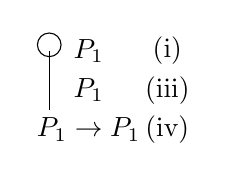
\begin{tikzpicture}[scale=0.5]
            \begin{scope}[xshift=25cm]
                \draw (1,2) -- (1,0.5);
                \draw (1,2.15) circle (0.3cm);
                \node at (2,2) {$P_1$};
                \node at (4,2) {(i)};
                \node at (2,1) {$P_1$};
                \node at (4,1) {(iii)};
                \node at (2,0) {$P_1 \rightarrow P_1$};
                \node at (4,0) {(iv)};
            \end{scope}
        \end{tikzpicture}
        \caption{$P_1 \rightarrow P_1$的证明}
    \end{figure}
\end{example}

\begin{example}
    证明:$(\neg P_1) \rightarrow (P_1 \rightarrow P_2)$
    \begin{figure}[h]
        \centering
        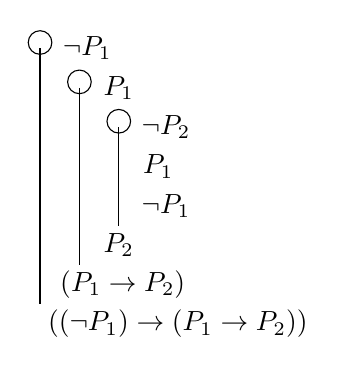
\begin{tikzpicture}[scale=0.5]
            \begin{scope}[xshift=25cm]
                \draw (1,7) -- (1,0.5);
                \draw (1,7.15) circle (0.3cm);
                \node at (2.2,7) {$\neg P_1$};
                \node at (3,6) {$P_1$};
                \draw (2,6) -- (2,1.5);
                \draw (2,6.15) circle (0.3cm);
                \node at (4.2,5) {$\neg P_2$};
                \draw (3,5) -- (3,2.5);
                \node at (4,4) {$P_1$};
                \node at (4.2,3) {$\neg P_1$};
                \node at (3,2) {$P_2$};
                \node at (3.1,1) {$(P_1 \rightarrow P_2)$};
                \draw (3,5.15) circle (0.3cm);
                \node at (4.5,0) {$((\neg P_1) \rightarrow (P_1 \rightarrow P_2))$};
            \end{scope}
        \end{tikzpicture}
        \caption{$(\neg P_1) \rightarrow (P_1 \rightarrow P_2)$的证明}
    \end{figure}
\end{example}

\newpage
再同理可以证明L1、L2、L3的正确性,从而可以证明命题演算的自然推演系统C与命题演算的公理系统L等价,即二者的定理集完全相同。

\begin{note}
    更一般的自然演绎系统常常含有合取、析取、等值等推演规则,一般的推演规则也不仅仅有这6条。
\end{note}

\chapter{基本命题的结构,词项}\label{chap5}

前面的章节(\ref{chap2,chap3,chap4})介绍了复合命题及其推理,讲述了有效推理形式的判定和生成。下面我们将目光放在基本命题\index{基本命题}上,研究单个命题本身的组成。

\begin{example}
    考虑这样一个例子:

    $$\text{凡星期四有课} \land \text{今天是星期四} \rightarrow \text{今天有课}$$

    这个推理不能用前几章的内容解释:$(P_1 \land P_2)\rightarrow P_3$。
\end{example}
基本命题内部的结构导致了这个推理是正确的,我们需要打开这些命题来研究推理的合理性。

\section{基本命题的结构}

\begin{itemize}[itemsep=0pt,parsep=0pt]
    \item \textbf{谓词}\index{谓词}:谓语部分,表达了事情是什么情况;
    \item \textbf{主词}\index{主词}:主语部分;
    \item \textbf{量词}\index{量词}:全体或一部分。
\end{itemize}

\begin{example}
    一些基本命题:

    ·有的人会游泳

    ·所有人要饮食

    其中“有的”“所有”就是量词。
\end{example}

量词是\textbf{逻辑常项}\index{逻辑常项}。

谓词和主词是\textbf{逻辑变项}\index{逻辑变项},充当谓词和主词的是\textbf{词项}\index{词项}。

\section{词项的内涵和外延}

\begin{note}
    在旧教科书中,“命题”被称为“概念”,有时词项的内涵与外延也被称作“概念的内涵与外延”。
\end{note}

\begin{itemize}[itemsep=0pt,parsep=0pt]
    \item \textbf{内涵}\index{内涵}:某一词项的含义,即该词项对象共同的特有属性。
    \item \textbf{外延}\index{外延}:某一词项所指称的对象。
\end{itemize}

内涵和外延之间有\textbf{反变关系}。

\begin{note}
    举例:

    \textbf{内涵:}内涵是指一个概念所包含的所有属性或特征。例如,“鸟”这个概念的内涵可能包括“有羽毛”、“能飞行”、“有喙”等特征。

    \textbf{外延:}外延是指一个概念所能适用的所有具体实例或个体。例如,“鸟”这个概念的外延包括所有的鸟类,如“麻雀”、“鹦鹉”、“鸽子”等。

    \textbf{反变关系:}当我们增加一个概念的内涵时,例如将“鸟”的定义改为“有羽毛、能飞行、有喙,并且是猛禽”,那么这个概念的外延就会减少,因为不是所有的鸟都是猛禽。反之,如果我们减少概念的内涵,例如将“鸟”的定义改为“有羽毛”,那么这个概念的外延就会增加,因为有羽毛的动物不仅包括鸟,还可能包括其他动物,如某些恐龙种类。

    内涵和外延之间的关系是一种反变关系,一个增加另一个就会减少,反之亦然。
\end{note}

\begin{itemize}[itemsep=0pt,parsep=0pt]
    \item 词项的\textbf{限制}:增加词项的内涵以缩小外延;
    \item 词项的\textbf{扩大}:减少词项的内涵以扩大外延。
\end{itemize}

\section{词项的种类}

根据词项外延的数量情况,词项分为:
\begin{itemize}[itemsep=0pt,parsep=0pt]
    \item \textbf{普遍词项}\index{普通词项}:外延超过一个;
    \item \textbf{单独词项}\index{单独词项}:外延只有一个;
    \item \textbf{空词项}\index{空词项}:外延为空。
\end{itemize}

\begin{example}
    一些例子:
    \begin{itemize}[itemsep=0pt,parsep=0pt]
        \item \textbf{普遍词项}:这种词项的外延超过一个,也就是说,它可以指代多个实体。例如,“动物”这个词项的外延包括所有的动物,如“狗”、“猫”、“鸟”等。
        \item \textbf{单独词项}:这种词项的外延只有一个,也就是说,它只指代一个特定的实体。例如,“埃菲尔铁塔”这个词项的外延就是埃菲尔铁塔这个具体的建筑物。
        \item \textbf{空词项}:这种词项的外延为空,也就是说,它不指代任何实体。例如,“方圆形”这个词项的外延为空,因为没有任何实体既是方的又是圆的。
    \end{itemize}
\end{example}

\section{词项间的关系}

指词项外延间的关系:
\begin{itemize}[itemsep=0pt,parsep=0pt]
    \item \textbf{全同(同一)关系}\index{全同关系}:两个集合完全重合。
    \item \textbf{包含关系和包含于关系}\index{包含关系,包含于关系}:一个集合完全包含在另一个集合中。
    \item \textbf{交叉关系}\index{交叉关系}:两个集合有一部分重叠。
    \item \textbf{全异关系}\index{全异关系}:
    \begin{itemize}[itemsep=0pt,parsep=0pt]
        \item \textbf{矛盾关系}\index{矛盾关系}:两个集合没有任何交集。
        \item \textbf{反对关系}\index{反对关系}:两个集合的并集等于全集,交集不为空。
    \end{itemize}
\end{itemize}
Euler图是他们关系之间的展示。

\begin{figure}[h]
    \centering
    \begin{subfigure}{.5\textwidth}
      \centering
      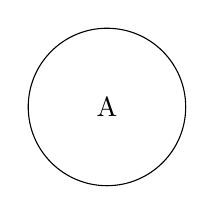
\begin{tikzpicture}
      \draw (0,0) circle (1cm);
      \node at (0,0) {A};
      \end{tikzpicture}
      \caption{全同(同一)关系}
    \end{subfigure}%
    \begin{subfigure}{.5\textwidth}
      \centering
      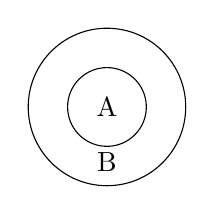
\begin{tikzpicture}
        \draw (0,0) circle (1cm);
        \node at (0,0) {A};
        \draw (0,0) circle (0.5cm);
        \node at (0,-0.7) {B};
      \end{tikzpicture}
      \caption{包含关系和包含于关系}
    \end{subfigure}
    \begin{subfigure}{.5\textwidth}
      \centering
      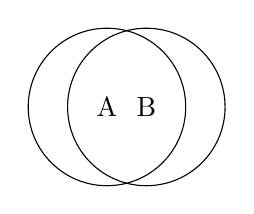
\begin{tikzpicture}
      \draw (0,0) circle (1cm) node {A};
      \draw (0.5,0) circle (1cm) node {B};
      \end{tikzpicture}
      \caption{交叉关系}
    \end{subfigure}%
    \begin{subfigure}{.5\textwidth}
      \centering
      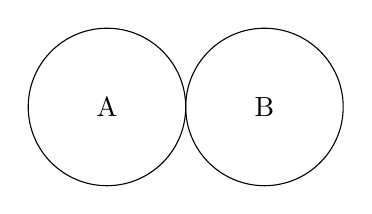
\begin{tikzpicture}
      \draw (0,0) circle (1cm) node {A};
      \draw (2,0) circle (1cm) node {B};
      \end{tikzpicture}
      \caption{全异关系:矛盾关系}
    \end{subfigure}
    \begin{subfigure}{.5\textwidth}
      \centering
      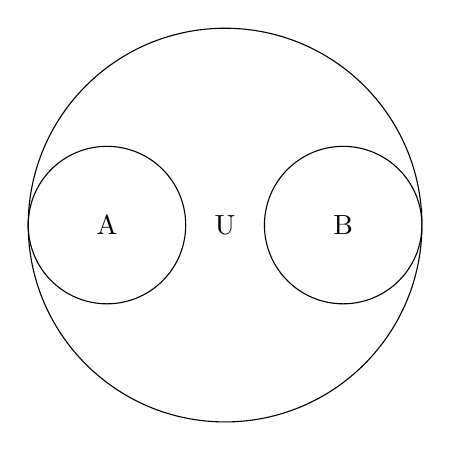
\begin{tikzpicture}
      \draw (-1.5,0) circle (1cm) node {A};
      \draw (1.5,0) circle (1cm) node {B};
      \draw (0,0) circle (2.5cm) node {U};
      \end{tikzpicture}
      \caption{全异关系:反对关系}
    \end{subfigure}
    \caption{词项外延间的Euler图}
\end{figure}

\newpage

\section{词项的定义}

\textbf{定义}\index{定义}的定义:描述词项的内涵。

\textbf{定义}的结构:被定义项,定义项。

\textbf{定义}的主要规则:定义项和被定义项须为全同关系;定义项不得直接或间接包含被定义项。

\begin{example}
    我们对主要规则做一解释:
    \begin{itemize}[itemsep=0pt,parsep=0pt]
        \item 鱼是可以在水下生活的生物。
        
        这样的定义是不合法的,因为不满足全同关系。

        \item 逻辑学是研究逻辑的学科。
        
        这样的定义是不合法的,因为定义中直接包含了被定义项。

        \item 三教的位置在六教西边;六教的位置在三教东边。
        
        这样的定义是不合法的,因为在循环定义项间接包含了被定义项。
    \end{itemize}
\end{example}

定义一定要有出发点,即不被定义的东西(被称为\textbf{初始符号},例如$\neg ,\rightarrow$),否则会陷入循环定义的闭环。

\section{词项的划分}

\textbf{划分}\index{划分}:分类列举词项的外延。

\textbf{划分}的结构:母项,子项。

\textbf{划分}的主要规则:每一外延应属于某一子项并只属于一个子项。即:
\begin{itemize}[itemsep=0pt,parsep=0pt]
    \item 子项相加应恰等于母项,不得遗漏;
    \item 子项之间应互相排斥,不得重合。
\end{itemize}

\chapter{性质命题的推理}\label{chap6}

\section{一元谓词和多元谓词}

回顾前面(第\ref{chap5}章)的命题结构的分析:

\begin{itemize}[itemsep=0pt,parsep=0pt]
    \item 谓词:谓语部分,表达了事情是什么情况;
    \item 主词:主语部分;
    \item 量词:全体或一部分。
\end{itemize}

\textbf{一元谓词}\index{一元谓词}:每次需要一个主词与之配合,通常表示某种性质;

\textbf{多元(如二元,三元,......)谓词}\index{多元谓词}:每次需要多个(如两个,三个,......)主词与之配合,通常表示某种关系。

\textbf{性质命题}\index{性质命题}:含有一元谓词的基本命题;

\textbf{关系命题}\index{关系命题}:含有多元谓词的基本命题。

每个基本命题包含:
\begin{itemize}[itemsep=0pt,parsep=0pt]
    \item 谓词:一个,
    \item 主词:个数与谓词的元数相应,每个主词可有相应的量词。
\end{itemize}

\begin{example}
    一元谓词性质命题

    “张三和李四是学生。”——谓词“是学生”:一元谓词。

    可以理解为复合命题,包含两个基本命题(性质命题):

    “张三是学生”(主词:张三)和“李四是学生”(主词:李四)。
\end{example}

\begin{example}
    多元谓词关系命题

    “张三和李四是邻居。”——谓词“是邻居”:二元谓词。
    
    一个基本命题(关系命题)(主词:“张三”、“李四”)。
\end{example}

\begin{example}
    多元谓词关系命题

    5>3:“5”与“3”都是主词,大于是关系。
\end{example}

关系命题的谓词一般表示关系。

\section{传统逻辑对性质命题的分析}

\textbf{数理逻辑的分析:}

\begin{tabular}{ccccc}
    昨天&下雨。&今天&不&下雨。\\
    &&&↓&\\
    \underline{昨天}&\underline{下雨}。&\underline{并非}&\underline{今天}&\underline{下雨}。\\
    主词&谓词&命题联结词&主词&谓词\\
\end{tabular}

\textbf{传统逻辑的分析:}

\begin{tabular}{cccccc}
    昨天&&下雨。&今天&不&下雨。\\
    &&&↓&\\
    \underline{昨天}&\underline{(是)}&\underline{下雨}。&\underline{今天}&\underline{不}&\underline{下雨}。\\
    主词&联词&谓词&主词&联词&谓词\\
\end{tabular}

传统逻辑中,往往把“否定”分析为在性质命题内部与“肯定”相对的成分。“肯定”和“否定”称为\textbf{联词}\index{联词},表明主词和谓词之间具有肯定的联系或否定的联系。

数理逻辑中我们默认主词和谓词之间只有肯定的联系。传统逻辑要比数理逻辑多一个成分——联词。

\textbf{传统逻辑对性质命题的分析:}

主词(S),谓词(P),量词,联词。

量词和联词为\textbf{逻辑常项}。

\subsection{逻辑常项}\index{逻辑常项}

\subsubsection{量词}

\begin{itemize}[itemsep=0pt,parsep=0pt]
    \item \textbf{全称}\index{全称量词}:主词有不止一个外延,每个外延都和谓词之间有相应的联系;
    \item \textbf{特称(存在)}\index{特称量词}:主词外延不止一个,存在外延和谓词之间有相应的联系;
    \item \textbf{单称}\index{单称量词}:主词只有一个外延,外延和谓词之间有相应联系。
\end{itemize}

\begin{example}
    量词的使用举例
    \begin{itemize}[itemsep=0pt,parsep=0pt]
        \item 全称:“人要吃饭。”
        
        \emph{全称量词可省略。}
        \item 存在、特称:“有的人会游泳。”
        
        \emph{特称(存在)量词的含义:至少存在一个(不排斥全部)}。

        但注意“有的”应不含“有的没有”的意义。应表示“至少存在一个”,无关“有的不存在”的意思。

        即上面的例子不能含有“有的人不会游泳。”的含义。日常语言中“有”更符合存在量词的意义。
        \item 单称:“北京大学是世一大。”
        
        可以说“所有北京大学”、“这个北京大学”。

        \emph{单称量词通常处理为全称。}
    \end{itemize}
\end{example}

\subsubsection{联词}

\begin{itemize}[itemsep=0pt,parsep=0pt]
    \item 肯定
    \item 否定
\end{itemize}

肯定联词可省略。

\section{性质命题的种类}

根据命题中\textbf{逻辑常项}的组合,性质命题分为:

\begin{itemize}[itemsep=0pt,parsep=0pt]
    \item \textbf{全称肯定(SAP)}\index{SAP}:所有S是P
    \item \textbf{全称否定(SEP)}\index{SEP}:所有S不是P
    \item \textbf{特称肯定(SIP)}\index{SIP}:有S是P
    \item \textbf{特称否定(SOP)}\index{SOP}:有S不是P
\end{itemize}

\section{性质命题中主、谓词的周延}

\textbf{周延:}\index{周延}词项出现在性质命题中时,是否涉及到其全部外延,称为是否周延。

\begin{center}
    \begin{tabular}{ll}
        \underline{S}AP:&所有S是P\\

        \underline{S}E\underline{P}:&所有S不是P\\

        SIP:&有S是P\\

        SO\underline{P}:&有S不是P\\
    \end{tabular}   
\end{center}

全称命题(A、E)的主词周延,特称命题(I、O)的主词不周延。

否定命题(E、O)的谓词周延,肯定命题(A、I)的谓词不周延。

\begin{note}
    周延的举例:

    (A)“所有的人类都是哺乳动物”。
    
    在这个命题中,主词是“人类”,谓词是“哺乳动物”,这个命题的主词周延、谓词不周延。
    
    “人类”能代表所有人,涉及到了人类的所有外延;“哺乳动物”这里虽然没有使用量词,但是由于全句是肯定判断,所以其外延是“无穷大”的。这时候称作人类的哺乳动物也只是所有哺乳动物中的一部分,因此“哺乳动物”是不周延概念。

    换句话讲,由于人类$\subsetneqq$哺乳动物,而哺乳动物还有其他外延,所以不周延。

    (E)“所有的狗都不会飞行”即“所有的狗都不是会飞行的动物”。
    
    在这个命题中,谓词是“会飞行的动物”。这个命题的谓词周延,因为对于“所有”“会飞行的动物”,狗都不在里面。

    其实是说,如果能给这个词项前面加上“所有”而意思不变,那么这个词项所有的外延都被涉及到,也就是这个词项是周延的。
\end{note}

\textbf{关于词项周延的一般规则:}

推理中,在前提中出现时不周延的词项,在结论中出现时也不得周延。

\section{命题变形的推理}

换位法:

\begin{center}
    \begin{tabular}{lll}
        \underline{S}E\underline{P}&$\Rightarrow$&\underline{P}E\underline{S}\\

        SIP&$\Rightarrow$&PIS\\

        \underline{S}AP &$\Rightarrow$& PA\underline{S} ×\\

        SO\underline{P}&$\Rightarrow$&\underline{P}OS ×\\
    \end{tabular}   
\end{center}

推理中,在前提中出现时不周延的词项,在结论中出现时也不得周延。

但可以有这样的推理:

\begin{center}
SAP$ \Rightarrow$ PIS
\end{center}

\section{根据对当关系的推理}

\textbf{逻辑方阵}\index{对当关系}
\begin{enumerate}[itemsep=0pt,parsep=0pt]
    \item \textbf{反对关系}\index{反对关系}(SAP与SEP):可以同假,不能同真;
    \item \textbf{下反对关系}\index{下反对关系}(SIP与SOP):可以同真,不能同假;
    \item \textbf{矛盾关系}\index{矛盾关系}(SAP与SOP,SEP与SIP):必一真一假;
    \item \textbf{差等关系}\index{差等关系}(SAP对SIP,SEP对SOP):全称真则特称必真,特称假则全称必假。
\end{enumerate}

\begin{figure}
    \begin{center}
    \begin{tikzpicture}[
        node distance=3cm,
        every node/.style={minimum size=1cm}]
        
        \node (A) at (0,0) {A};
        \node (I) at (0,-4) {I};
        \node (E) at (4,0) {E};
        \node (O) at (4,-4) {O};
        
        \draw[-] (A) to node [above, midway] {反对} (E);
        \draw[-] (I) to node [below, midway] {下反对} (O);
        \draw[-] (A) to node [left, midway] {矛盾} (I);
        \draw[-] (E) to node [right, midway] {矛盾} (O);
        \draw[dashed] (A) -- (O) node[midway,sloped,above]{};
        \draw[dashed] (E) -- (I) node[midway,below]{差等};
        
    \end{tikzpicture}
    \caption{对当关系的逻辑方阵}
    \end{center}
\end{figure}

\begin{table}
    \begin{center}
    \begin{tabular}{c:c:c}
        \begin{tabular}{lll}
            SAP  &$\Rightarrow$&$¬$ (SEP)\\
            &$\Rightarrow$&SIP\\
            &$\Rightarrow$&$¬$ (SOP)
        \end{tabular} &
        \begin{tabular}{lll}
            $¬$ (SAP) &$\Rightarrow$&SOP\\
            &&\\
            &&
        \end{tabular} &
        \begin{tabular}{lll}
            SEP  &$\Rightarrow$&$¬$ (SAP)\\
            &$\Rightarrow$&$¬$ (SIP)\\
            &$\Rightarrow$&SOP 
        \end{tabular} \\ 
        \hdashline
        \begin{tabular}{lll}
            $¬$ (SEP) &$\Rightarrow$&SIP\\
            &&\\
            &&
        \end{tabular} &
        \begin{tabular}{lll}
            SIP  &$\Rightarrow$&$¬$ (SEP)\\
            &&\\
            &&
        \end{tabular} &
        \begin{tabular}{lll}
            $¬$ (SIP) &$\Rightarrow$&$¬$ (SAP)\\
            &$\Rightarrow$&SEP\\
            &$\Rightarrow$&SOP 
        \end{tabular} \\
        \hdashline
        \begin{tabular}{lll}
            SOP  &$\Rightarrow$& (SAP)\\
            &&\\
            &&
        \end{tabular} &
        \begin{tabular}{lll}
            $¬$(SOP) &$\Rightarrow$&SAP\\
            &$\Rightarrow$&$¬$ (SEP)\\
            &$\Rightarrow$&SIP 
        \end{tabular} &
        \\ 
    \end{tabular}
    \caption{根据对当关系的推理}
    \end{center}
\end{table}

\section{三段论}

\subsection{三段论(syllogism)}

\textbf{三段论}\index{三段论}:由包含一个共同词项的两个性质命题作为前提,推出一个性质命题作为结论。

\subsection{三段论的结构}

作为结论之主词的词项:\textbf{小词(S)}\index{小词}

作为结论之谓词的词项:\textbf{大词(P)}\index{大词}

只出现在前提中的词项:\textbf{中词(M)}\index{中词}

含有大词的前提:\textbf{大前提}\index{大前提}

含有小词的前提:\textbf{小前提}\index{小前提}

\begin{table}[h]
\begin{center}
    \begin{tabular}{l|l}
    凡星期四(M)都有课(P)&凡星期四(P)都有课(M)\\
    今天(S)是星期四(M)&今天(S)有课(M)\\
    \hdashline
    今天(S)有课(P)&今天(S)是星期四(P)\\
    \end{tabular}
    \caption{三段论的结构}
\end{center}
\end{table}

\subsection{三段论的式与格}

\subsubsection{式}
\textbf{式:}\index{式}由分别作为大前提、小前提、结论的性质命题的种类而确定。共有$4^3=64$个式。

例如:

\begin{table}[h]
\begin{center}
\begin{tabular}{l|l}
凡星期四都有课\textcolor{red}{A} &凡星期四都有课\textcolor{red}{A}\\
今天是星期四\textcolor{red}{A}   &  今天有课\textcolor{red}{A}\\
\hdashline
今天有课\textcolor{red}{A}  &   今天是星期四\textcolor{red}{A}\\
\hline
\textcolor{red}{AAA式}&\textcolor{red}{AAA式}\\
\end{tabular}
\par
\begin{tabular}{l|l}
凡星期四都有课\textcolor{red}{A}  &  凡星期四都有课\textcolor{red}{A}\\
今天不是星期四\textcolor{red}{E}   &    今天没课\textcolor{red}{E}\\
\hdashline
今天没课\textcolor{red}{E}  & 今天不是星期四\textcolor{red}{E}  \\
\hline
\textcolor{red}{AEE式}&\textcolor{red}{AEE式}\\
\end{tabular}
\caption{三段论的式举例}
\end{center}
\end{table}

\subsubsection{格}
\textbf{格:}由中词、大词、小词在前提中的位置而确定,共有4个格。

\begin{table}[h]
\begin{center}
    \begin{tabular}{c|c|c|c}
        第1格&第2格&第3格&第4格\\
        \hline
        M—P&P—M&M—P&P—M\\
        S—M&S—M&M—S&M—S\\
        \hdashline
        S—P&S—P&S—P&S—P\\
    \end{tabular}
    \caption{三段论的格}
\end{center}
\end{table}

\begin{table}[h]
\begin{center}
    \begin{tabular}{l|l}
        凡星期四(\textcolor{blue}{M})都有课(\textcolor{blue}{P})\textcolor{red}{A}& 凡星期四(\textcolor{blue}{P})都有课(\textcolor{blue}{M})\textcolor{red}{A}\\
        今天(\textcolor{blue}{S})是星期四(\textcolor{blue}{M})\textcolor{red}{A} & 今天(\textcolor{blue}{S})有课(\textcolor{blue}{M})\textcolor{red}{A}\\
        \hdashline
        今天(\textcolor{blue}{S})有课(\textcolor{blue}{P})\textcolor{red}{A} & 今天(\textcolor{blue}{S})是星期四(\textcolor{blue}{P})A\\
        \hline
        \textcolor{red}{AAA}-\textcolor{blue}{1}&\textcolor{red}{AAA}-\textcolor{blue}{2}\\
        \hline
        凡星期四(\textcolor{blue}{M})都有课(\textcolor{blue}{P})\textcolor{red}{A} & 凡星期四(\textcolor{blue}{P})都有课(\textcolor{blue}{M})\textcolor{red}{A}\\
        今天(\textcolor{blue}{S})不是星期四(\textcolor{blue}{M})\textcolor{red}{E} & 今天(\textcolor{blue}{S})没课(\textcolor{blue}{M})\textcolor{red}{E}\\
        \hdashline
        今天(\textcolor{blue}{S})没课(\textcolor{blue}{P})\textcolor{red}{E} &今天(\textcolor{blue}{S})不是星期四(v\textcolor{blue}{P})\textcolor{red}{E}\\
        \hline
        \textcolor{red}{AEE}-\textcolor{blue}{1}&\textcolor{red}{AEE}-\textcolor{blue}{2}\\
    \end{tabular}
    \caption{三段论的格举例}
\end{center}
\end{table}

三段论共有$64\cdot4=256$种可能的格。

\subsection{三段论有效格式的规则}

写成三段论的标准形式之后:

\begin{enumerate}[itemsep=0pt,parsep=0pt]
\item 中词在前提中至少周延一次:

如果中项一次都不周延,那它就没法起到桥梁的作用,将S和P联系起来。

\item 前提与结论中,二者否定命题的数量相等:

两个肯定命题得出肯定命题作为结论,一个肯定、一个否定命题得出否定命题作为结论,两个否定命题不能得出结论。

\item 小词、大词在结论中若周延,则其在前提中必须周延。
\item (Bool观点)两个全称命题作为前提,推不出特称命题的结论:

在Bool看来,全称命题没有存在性预设,而特称命题有。前提中没有的东西,结论中不能有。结论中有的东西,前提中必然也要有。结论不能比前提更强。

\end{enumerate}

\begin{table}[h]
\begin{center}
    \begin{tabular}{l|l}
        凡\underline{星期四(M)}都有课(P)A&凡\underline{星期四(P)}都有课(M)A\\
        \underline{今天(S)}是星期四(M)A&\underline{今天(S)}有课(M)A\\
        \hdashline
        \underline{ 今天(S)}有课(P)A&\underline{今天(S)}是星期四(P)A\\
        \hline
        AAA-1      &               AAA-2  \textcolor{green}{无效:中词没有周延}\\
        \hline
        凡\underline{星期四(M)}都有课(P)A &凡\underline{星期四(P)}都有课(M)A\\
        \underline{今天(S)}不是\underline{星期四(M)}E&\underline{今天(S)}没\underline{课(M)}E\\
        \hdashline
        \underline{今天(S)}没\underline{课(P)}E & \underline{今天(S)}不是\underline{星期四(P)}E\\
        \hline
        AEE-1 \textcolor{green}{无效:大前提没有周延}&AEE-2\\
    \end{tabular}
    \caption{三段论的有效格式举例}
\end{center}
\end{table}

\begin{example}
    又如:
\begin{center}
\begin{tabular}{l}
鲁迅的著作(M1)不能一天读完(P)\\
《祝福》(S)是鲁迅的著作(M2)\\
\hdashline
《祝福》(S)不能一天读完(P)\\
\end{tabular}
\end{center}
“鲁迅的著作(M1)”和“鲁迅的著作(M2)”并非共同词项,这不是三段论。
\end{example}

\textbf{三段论的有效格式:}
\begin{table}[h]
    \begin{center}
    \begin{tabular}{c:c:c:cc}
        第一格&第二格&第三格&第四格&\\
        AAA & AEE & AAI & AAI&\\
        AII & EAE & AII & AEE&\\
        EAE & EIO & EAO & EAO&\\
        EIO & AOO & EIO & EIO&\\
        (AAI) & (AEO) & IAI & IAI&\\
        (EAO) & (EAO) & OAO & (AEO)&(弱式)
    \end{tabular}
    \caption{三段论的有效格式}
\end{center}
\end{table}

\newpage

\section{性质命题在数理逻辑中的表述}\label{feikong}

一个命题用以下方式表达:$P(x):x\text{是}P$。其中$P$:谓词变元(谓词),$x$:个体变元(主词),量词:任意、存在。

两个量词可以互相替换:

$$(\forall x)(P(x)) \Leftrightarrow \neg(\exists x)\neg(P(x))$$
$$(\exists x)(P(x)) \Leftrightarrow \neg(\forall x)\neg(P(x))$$

如果考虑个体变元的\textbf{论域}:

全称肯定(SAP):所有S是P
$$((\forall x)(S(x)\rightarrow P(x)))$$

全称否定(SEP):所有S不是P
$$((\forall x)(S(x)\rightarrow (\neg P(x))))$$

特称肯定(SIP):有S是P
$$((\exists x)(S(x)\wedge P(x)))$$

特称否定(SOP):有S不是P
$$((\exists x)(S(x)\wedge (\neg P(x))))$$

\section{主词非空的预设}
考虑上文的对当关系的图,例如SAP与SIP是等差关系。


\begin{tabular}{ll}
    $((\forall x)(S(x)\rightarrow P(x)))$& A命题\\
    推出&由A命题推出I命题\\
    $((\exists x)(S(x)\wedge P(x)))$&I命题\\
    再推出& 由(p$\wedge$ q)推出p\\
    $((\exists x)(S(x)))$&\\
\end{tabular}

但这样的推理有问题。

\begin{example}
    上述例子的一个实例是:

    “如果有妖怪的话我都不害怕”推出“存在妖怪”。
\end{example}

若想从A命题推出I命题,必须增加前提$((\exists x)(S(x)))$
\begin{align*}
    ((\forall x)(S(x)\rightarrow P(x)))\wedge((\exists x)(S(x))) &\Rightarrow\\
    (\forall x)(S(x)\wedge P(x)) &\Rightarrow\\
    (\exists x)(S(x))
\end{align*}

由全称命题推出存在命题,要保证主词S不能为空词项。

\begin{note}
    这是因为传统逻辑不考虑主词为空词项的情况。
\end{note}

\chapter{关系命题的推理}\label{chap7}

\section{关系命题的结构}

\textbf{关系命题:}\index{关系命题}含有多元谓词的基本命题。

例如二元关系命题:$R(x,y):x\text{对于}y\text{,有关系}R$。其中$R$:谓词变元,$x,y$:个体变元,量词:任意、存在。

有以下八种二元关系命题:

$(\forall x)(\forall y)R(x,y)$:所有老鼠怕所有的猫

$(\forall y)(\forall x)R(x,y)$:所有猫被所有老鼠怕

$(\forall x)(\exists y)R(x,y)$:对于每一个老鼠,都有一个猫是它害怕的

$(\exists y)(\forall x)R(x,y)$:存在一个猫被所有老鼠害怕

$(\exists x)(\forall y)R(x,y)$:存在一个老鼠害怕所有猫

$(\forall y)(\exists x)R(x,y)$:对于任意的猫,存在一个老鼠害怕他

$(\exists x)(\exists y)R(x,y)$:存在一个老鼠,有一个猫被他害怕

$(\exists y)(\exists x)R(x,y)$:存在一个猫,有一个老鼠害怕他

\section{根据量词的推理}

存在量词可以往后放,特称量词可以往前放。全称可以推出特称。

\begin{center}
    \begin{tabular}{ccc}
        $(\forall x)(\forall y)R(x,y)$ &$\Leftrightarrow$&$(\forall y)(\forall x)R(x,y)$\\
        &$\Downarrow$&\\
        $(\forall x)(\exists y)R(x,y)$&$\Leftarrow$&$(\exists y)(\forall x)R(x,y)$\\
    
        $(\exists x)(\forall y)R(x,y)$&$\Rightarrow$&$(\forall y)(\exists x)R(x,y)$\\
        &$\Downarrow$&\\
        $(\exists x)(\exists y)R(x,y)$&$\Leftrightarrow$&$(\exists y)(\exists x)R(x,y)$
    \end{tabular}
\end{center}

\begin{note}
    正如上一章(\ref{feikong})所提到的,我们仍需要考虑非空词项的问题。
\end{note}

\section{根据谓词性质的推理}

二元关系常见的性质:
\begin{enumerate}[itemsep=0pt,parsep=0pt]
    \item 自返性
    \begin{enumerate}[itemsep=0pt,parsep=0pt]
        \item 自返关系:$(\forall x) R(x,x)$
        \item 反自返关系:$(\forall x)(¬R(x,x))$
        \item 非自返关系:$((\exists x)R(x,x))\wedge (\exists x)(\neg R(x,x))$
    \end{enumerate}
    \item 对称性
    \begin{enumerate}[itemsep=0pt,parsep=0pt]
        \item 对称关系:$(\forall x)(\forall y)((R(x,y))\Rightarrow(R(y,x)))$
        \item 反对称关系:$(\forall x)(\forall y)((R(x,y))\Rightarrow(¬R(y,x)))$
        \item 非对称关系:$((\exists x)(\exists y)((R(x,y))\Rightarrow(R(y,x))))$
        
        $\wedge((\exists x)(\exists y)((R(x,y))\Rightarrow(¬R(y,x))))$
    \end{enumerate}
    \item 传递性
    \begin{enumerate}[itemsep=0pt,parsep=0pt]
        \item 传递关系:$(\forall x)(\forall y)(\forall z)(((R(x,y)∧R(y,z)))\Rightarrow R(x,z))$
        \item 反传递关系:$(\forall x)(\forall y)(\forall z)(((R(x,y)∧R(y,z)))\Rightarrow(¬R(x,z)))$
        \item 非对称关系:$((\exists x)(\exists y)(\exists z)(((R(x,y)∧R(y,z)))\Rightarrow R(x,z)))$
        
        $\wedge((\exists x)(\exists y)(\exists z)(((R(x,y)∧R(y,z)))\Rightarrow(¬R(x,z))))$
    \end{enumerate}
\end{enumerate}

必须注意:“根据谓词性质的推理”只是给出了一种方法,不是本来意义上纯形式的逻辑推理。只能看作这是对于一些性质结构在形式上的规定。

\chapter{*谓词演算概要}\label{chap8}


正如第\ref{chap4}章可以处理第\ref{chap2}章的复合命题的有效推理形式。

本章节的谓词演算系统可以处理前两章的内容。

\section{一阶语言}
用于谓词演算的形式语言。

符号表:

\begin{tabular}{ll}
    $x_1,x_2,…$ &变元\\
    $a_1,a_2,… $&个体常元\\
    $A_1^1 ,A_2^1 ,…; A_1^2 ,A_2^2 ,…; A_1^3 ,A_2^3 ,…; …$ &谓词字母\\
    $f_1^1 ,f_2^1 ,…; f_1^2 ,f_2^2 ,…; f_1^3 ,f_2^3 ,…; …$ &函词字母\\
    (,),, &标记符号\\
    $\neg$ , $\rightarrow $ &联结词\\
    $\forall $ &量词\\
\end{tabular}

\textbf{一阶语言L:} \index{一阶语言}

\begin{enumerate}
    \item 符号表 ($i = 1,2,…; n =1,2,…$):
    
    \begin{tabular}{l}
    变元: $x_i$\\
    个体常元: $a_i$\\
    谓词字母: $A_i^n$\\
    函词字母: $f_i^n$\\
    标记符号:(,),,\\
    联结词: $\neg$ , $\rightarrow $\\
    量词:$\forall $\\
    \end{tabular}
    \item 形成规则:
    
    \begin{enumerate}

        \item L 中的项:
        \begin{enumerate}
            \item 变元和个体常元是项;
            \item 若$f_i^n$是 L 中的函词字母,且$ t_i,…, t_n$是 L 中的项,则$f_i^n$($t_1, …, t_n $)是 L 中的项;
            \item 所有项由(i)和(ii)生成。
        \end{enumerate}

        \item L 中的原子公式:
        
        若  $A_j^k$是 L 中的谓词字母,且 $t_i ,…,t_k$是 L 中的项,则$A_j^k$($t_1,…,t_k$ )是 L 中的原子公式。

        \item L 中的合式公式:
        
        \begin{enumerate}
            \item L 的每一原子公式是 L 的合式公式;
            \item 若 A 和 B 是 L 的的合式公式,则$(\neg A)$ ,$(A→B)$和$((\forall x_i) A)$也是合式公式,这里 $x_i$是任一变元;
            \item L 的所有合式公式由(i)和(ii)生成。
        \end{enumerate}

        \item 其他符号的定义(A, B 为任意合式公式):

        $((\exists x_i) A)$ 定义为$(¬((\forall x_i)((¬A )))$ ,

        $(A\wedge B)$定义为$(¬(A→(¬B )))$,

        $(A\vee B)$定义为$((¬A)→B )$。
    \end{enumerate}
\end{enumerate}
\section{一阶语言的解释和赋值}

一阶语言 L 的一个\textbf{解释}I:\index{解释}
\begin{itemize}[itemsep=0pt,parsep=0pt]
    \item 一个非空集合 $D_I$(I 的论域)
    \item $D_I$ 中的一组特定元素($\overline{a_1} ,\overline{a_2} , …$),
    \item $D_I$ 上的一组函数($\overline{f_i^n} $, i>0, n>0),
    \item $D_I$ 上的一组关系($\overline{A_i^n} $, i>0, n>0)。
\end{itemize}

\begin{example}
    一阶语言 L 的一个解释 N(形式算术):
    
    $D_N : { 0,1,2, … }$;
    
    $\overline{a_1} : 0, \overline{a_2} : 1$;

    $\overline{f_1^1} :\text{后继}(+1),\overline{f_1^2}  :+ , \overline{f_2^2}  :*$;

    $\overline{A_1^1} :>0, \overline{A_1^2} :=, \overline{A_2^2} :>$。

    这和自然数的建立是如出一辙的。
\end{example}

一阶语言 L 的解释 I 中的一个\textbf{赋值} v :\index{赋值}

对 L 中的每个变元指定 $D_I$的一个元素。

\section{满足,真,逻辑有效}

L 的合式公式 A 在 L 的解释 I 中的一个赋值 v 下成真,称为 v \textbf{满足} A。否则称为 v \textbf{不满足}  A。

L 的合式公式 A 在 L 的解释 I 中,每个赋值都满足 A,称为 A 在 I 中\textbf{真}。

L 的合式公式 A 在 L 的解释 I 中,每个赋值都不满足 A,称为 A 在 I 中\textbf{假}。

L 的合式公式 A 在 L 的每一解释中都真,称为 A \textbf{逻辑有效}。

L 的合式公式 A 在 L 的每一解释中都假,称为 A \textbf{矛盾}。

\begin{note}
    一些举例:
    \begin{itemize}[itemsep=0pt,parsep=0pt]
        \item A 在 I 中真:

    A:$\forall x , (P(x) \lor Q(x))$

    I:解释中的赋值 $v$ 对于所有个体常量 $c$,$v(P(c)) = \text{True}$,$v(Q(c)) = \text{True}$

    解释:在这个解释中,对于任何个体常量 $c$,A 都成立,因为 $P(c)$ 和 $Q(c)$ 都被赋值为真。因此,A 在 I 中是真的。
    \item A 在 I 中假:

    A:$\exists x , (P(x) \land \lnot Q(x))$

    I:解释中的赋值 $v$ 对于所有个体常量 $c$,$v(P(c)) = \text{True}$,$v(Q(c)) = \text{False}$

    解释:在这个解释中,对于任何个体常量 $c$,A 都不成立,因为 $P(c)$ 是真的,但 $Q(c)$ 是假的。因此,A 在 I 中是假的。
    \item A 逻辑有效:

    A:$\forall x , (P(x) \rightarrow Q(x))$

    解释:在所有可能的解释中,A 都是真的。例如,无论 P(x) 和 Q(x) 的具体含义如何,只要 P(x) 成立,则 Q(x) 也成立。因此,A 是逻辑有效的。
    \item A 矛盾:

    A:$\forall x , (P(x) \land \lnot P(x))$

    解释:在所有可能的解释中,A 都是假的。因为 $P(x)$ 和 $\lnot P(x)$ 不能同时成立,所以 A 是矛盾的。
\end{itemize}
\end{note}


\section{一阶谓词演算的公理系统}

一阶谓词演算的公理系统 KL

公理模式:(A, B, C 是 L 的任意合式公式,$x_i$是任意变元)

\begin{tabular}{ll}
    K1&$(A→(B→A))$\\
    K2&$((A→(B→C))→((A→B)→(A→C)))$\\
    K3&$(((¬A)→(¬B))→(B→A))$\\
    K4&$((\forall x_i)A→A)$, 若 $x_i$不在 A 中自由出现\\
    K5&$((\forall x_i)A(x_i)→ A(t))$, 若 A ($x_i$)是 L 的合式公式,而 t 是 L 中的项,\\&它对于 A($x_i$) 中的 $x_i$是自由的\\
    K6&$(\forall x_i)(A→B) →(A→(\forall x_i)B)$, 若 A 不包含变元 $x_i$的自由出现\\
\end{tabular}

推演规则:

(1)分离规则:从 $A$ 和$(A→B )$,得出 $B$

(2)概括规则:从 $A$ 得出$(\forall x_i)A$

\begin{note}
    
一阶谓词演算(first-order logic)确实可以看作是命题逻辑(propositional logic)的扩展。一阶谓词演算引入了更为复杂的语义元素,如量词和谓词,这让它能够表示更多的逻辑关系。

命题逻辑主要处理的是无内部结构的整体语句或命题,只关注这些命题如何通过逻辑运算符(如“和”、“或”、“非”、“如果...那么...”等)组合起来,而不考虑命题内部的结构。因此,命题逻辑可以看作是一阶谓词演算的一部分,它对应于一阶谓词演算中所有的量词都已经被消去,只剩下命题常量和逻辑运算符的情况。

二者的区别体现在:

\begin{itemize}[itemsep=0pt,parsep=0pt]
    \item 表达能力:命题演算主要关注完整的语句或命题之间的逻辑关系,它只能处理简单的真假判断,不关心命题内部的结构,因此其表达能力相对有限。一阶谓词演算则更强大,它可以处理命题内部的结构,如个体、属性和关系等,这让它能表达更为复杂的逻辑关系。

    \item 完备性和一致性:命题演算和一阶谓词演算都有完备性和一致性,这是指对于任何有效的逻辑公式,都可以在它们的公理系统中证明其为真,而对于任何无效的逻辑公式,都无法在它们的公理系统中证明其为真。然而,这个性质在更高阶的逻辑系统中就不再成立,这就是著名的哥德尔不完备定理。
\end{itemize}
\end{note}


\chapter{非标准(非经典)逻辑初步}\label{chap9}

\textbf{古典(传统)逻辑}\index{古典逻辑}\index{传统逻辑}【classical/traditional logic】

数理逻辑之前,亚里士多德为代表的传统形式逻辑。

\textbf{经典(标准)逻辑}\index{经典逻辑}\index{标准逻辑}【classical/standard logic】

罗素、怀特海《数学原理》的数理逻辑,基于二值外延逻辑系统的命题演算和命题演算系统。

\textbf{非经典(非标准)逻辑}\index{非经典逻辑}\index{非标准逻辑}【non-classical logic】

不属于经典逻辑的现代逻辑学分支系统。

\section{多值逻辑(many-valued logic)}\index{多值逻辑}

命题的真值取值:\{0,1,2,...,n\},1为真、n为假。

或取:[0,1]之间的数值,0为真,1为假。

卢卡西维兹:《论三值逻辑》第一次提出了多值逻辑。

\begin{table}
    \begin{center}
    \begin{tabular}{ccccccc}
    \hline
    P & Q & $\neg$ P & P $\wedge$ Q & P $\vee$ Q & P $\rightarrow$ Q & P $\leftrightarrow$ Q \\
    \hline
    1 & 1 & 3 & 1 & 1 & 1 & 1 \\
    1 & 2 & 3 & 2 & 1 & 2 & 2 \\
    1 & 3 & 3 & 3 & 1 & 3 & 3 \\
    2 & 1 & 2 & 2 & 1 & 1 & 2 \\
    2 & 2 & 2 & 2 & 2 & 1 & 1 \\
    2 & 3 & 2 & 3 & 2 & 2 & 2 \\
    3 & 1 & 1 & 3 & 1 & 1 & 3 \\
    3 & 2 & 1 & 3 & 2 & 1 & 2 \\
    3 & 3 & 1 & 3 & 3 & 1 & 1 \\
    \hline
    \end{tabular}
    \end{center}
    \caption{三值逻辑的真值表}
\end{table}

\newpage

\begin{note}
    可见把中间值(2)去掉之后,这是符合原本的二值逻辑的。二值逻辑是多值逻辑的子系统。
\end{note}

\section{模糊逻辑(fuzzy logic)}\index{模糊逻辑}

扎德(1921-2017)于1965年提出模糊逻辑概念,模糊逻辑即无穷多连续值逻辑。

其真值为“隶属度”,在$[0,1]$之间连续取值。

\begin{example}
    对于主词的任意取值,都有$[0,1]$之间的取值与之对应,这就可以画出一个曲线,来表示它的隶属度曲线。
\end{example}

\begin{figure}
    \begin{center}
    \begin{tikzpicture}
    \begin{axis}[
        % title={隶属度函数: 青年},
        xlabel={岁数},
        ylabel={隶属度},
        xmin=0, xmax=100,
        ymin=0, ymax=1.2,
        xtick={0,20,40,60,80,100},
        ytick={0,0.2,0.4,0.6,0.8,1},
        legend pos=north west,
        ymajorgrids=true,
        grid style=dashed,
    ]
     
    \addplot[
        color=blue,
        ]
        coordinates {
        (0,0)(10,0)(18,1)(25,1)(40,0.5)(60,0)(80,0)(100,0)
        };
    \legend{青年}
    
    \end{axis}
    \end{tikzpicture}
    \caption{隶属度函数: 青年}
    \end{center}
\end{figure}


\begin{note}
    曾被称作弗晰逻辑,是fuzzy的音译。但模糊逻辑并不是真值不确定的逻辑,而是无穷多连续值逻辑。
\end{note}

\newpage

\section{模态逻辑(modal logic)}\index{模态逻辑}

含有必然、可能等\textbf{模态(model)词}\index{模态词}的命题及其推论。

亚里士多德的模态三段论。

刘易斯(1883-1964)于1914年构造模态命题演算系统。

\textbf{基本模态词:}必然($\square$)与或然($\Diamond$)

根据模态命题之间的矛盾关系:

“必然”与“不可能不”等值,

“可能”与“不必然不”等值,

“不必然”与“可能不”等值,

“不可能”与“必然不”等值。

模态逻辑的逻辑方阵:

\begin{figure}[h]
    \begin{center}
    \begin{tikzpicture}[
        node distance=3cm,
        every node/.style={minimum size=1cm}]
        
        \node (A) at (0,0) {$\square P$};
        \node (I) at (0,-4) {$\Diamond P$};
        \node (E) at (4,0) {$\square \neg P$};
        \node (O) at (4,-4) {$\Diamond \neg P$};
        
        \draw[-] (A) to node [above, midway] {} (E);
        \draw[-] (I) to node [below, midway] {} (O);
        \draw[-] (A) to node [left, midway] {} (I);
        \draw[-] (E) to node [right, midway] {} (O);
        \draw[dashed] (A) -- (O) node[midway,sloped,above]{};
        \draw[dashed] (E) -- (I) node[midway,below]{};
        
    \end{tikzpicture}
    \caption{模态逻辑的逻辑方阵}
    \end{center}
\end{figure}

\newpage

不包含模态词的命题可以视为模态的特例:实然

模态逻辑的逻辑六边形:

\begin{figure}[h]
    \begin{center}
    \begin{tikzpicture}[
        node distance=3cm,
        every node/.style={minimum size=1cm}]
        
        \node (A) at (0,0) {$\square P$};
        \node (I) at (0,-4) {$\Diamond P$};
        \node (E) at (4,0) {$\square \neg P$};
        \node (O) at (4,-4) {$\Diamond \neg P$};
        \node (P) at (-2,-2) {$P$};
        \node (NotP) at (6,-2) {$\neg P$};
        
        \draw[-] (A) -- (E);
        \draw[-] (A) -- (P);
        \draw[-] (A) -- (I);
        \draw[-] (E) -- (O);
        \draw[-] (E) -- (NotP);
        \draw[-] (I) -- (O);
        \draw[-] (I) -- (P);
        \draw[-] (O) -- (NotP);
        \draw[-] (P) -- (NotP);
        \draw[-] (A) -- (O) node[midway,sloped,above]{};
        \draw[-] (E) -- (I) node[midway,below]{};
        
    \end{tikzpicture}
    \caption{模态逻辑的六边形}
    \end{center}
\end{figure}

\begin{note}
    同前面的多值逻辑,二值逻辑是模态逻辑的子系统。
\end{note}


\section{规范逻辑(normative logic)}\index{规范逻辑}

含有必须、允许等规范词的规范命题及其推理,亦称道义逻辑、义务逻辑等。

冯·赖特(1916-2003)于1951年发表《规范逻辑》,并创立规范逻辑系统。

基本规范词:必须O ,允许P,禁止(必须不)F。

规范逻辑的逻辑方阵:

\begin{figure}[h]
    \begin{center}
    \begin{tikzpicture}[
        node distance=3cm,
        every node/.style={minimum size=1cm}]
        
        \node (A) at (0,0) {$O P$};
        \node (I) at (0,-4) {$P P$};
        \node (E) at (4,0) {$F P$};
        \node (O) at (4,-4) {$P \neg P$};
        
        \draw[-] (A) to node [above, midway] {} (E);
        \draw[-] (I) to node [below, midway] {} (O);
        \draw[-] (A) to node [left, midway] {} (I);
        \draw[-] (E) to node [right, midway] {} (O);
        \draw[dashed] (A) -- (O) node[midway,sloped,above]{};
        \draw[dashed] (E) -- (I) node[midway,below]{};
        
    \end{tikzpicture}
    \caption{规范逻辑的逻辑方阵}
    \end{center}
\end{figure}
\begin{note}
    此系统中不能加入“实然”。这是主观上的要求,而非前面模态逻辑中客观的描述。

    就像“有人闯红灯”和“禁止闯红灯”是关系不大的。
\end{note}


\section{时态逻辑(tense logic)}\index{时态逻辑}

(普莱尔)基本时态词:永远,有时,某时。规范逻辑、时态逻辑等均属广义模态逻辑。

时态逻辑也能画出逻辑六边形:

\begin{figure}[h]
    \begin{center}
    \begin{tikzpicture}[
        node distance=3cm,
        every node/.style={minimum size=1cm}]
        
        \node (A) at (0,0) {永远};
        \node (I) at (0,-4) {有时};
        \node (E) at (4,0) {永远不};
        \node (O) at (4,-4) {有时不};
        \node (P) at (-2,-2) {某时};
        \node (NotP) at (6,-2) {某时不};
        
        \draw[-] (A) -- (E);
        \draw[-] (A) -- (P);
        \draw[-] (A) -- (I);
        \draw[-] (E) -- (O);
        \draw[-] (E) -- (NotP);
        \draw[-] (I) -- (O);
        \draw[-] (I) -- (P);
        \draw[-] (O) -- (NotP);
        \draw[-] (P) -- (NotP);
        \draw[-] (A) -- (O) node[midway,sloped,above]{};
        \draw[-] (E) -- (I) node[midway,below]{};
        
    \end{tikzpicture}
    \caption{模态逻辑的六边形}
    \end{center}
\end{figure}

\newpage

\begin{itemize}[itemsep=0pt,parsep=0pt]
    \item 反对(不能同真可以同假):
    
    永远p与永远$\neg$p,永远p与某时$\neg$p,永远$\neg$p与某时p
    \item 下反对(不能同假可以同真):
    
    有时p与有时$\neg$p,有时p与某时$\neg$p,有时$\neg$p与某时p
    \item 矛盾 (必一真一假):
    
    永远p与有时$\neg$p,永远$\neg$p与有时p,某时p与某时$\neg$p
    \item 差等(上真下必真,下假上必假):
    
    永远p对有时p,永远p对某时p,某时p对有时p;
    
    永远$\neg$p对有时$\neg$p,永远$\neg$p对某时$\neg$p,某时$\neg$p对有时$\neg$p
\end{itemize}

\begin{note}
    时态命题中可引入模态命题,构成时态模态命题。
\end{note}
\begin{note}
    规范逻辑、时态逻辑都属于广义模态逻辑。
\end{note}

\section{弗协调逻辑(paraconsistent logic)}\index{弗协调逻辑}

\begin{note}
    一般而言,非经典逻辑都是兼容经典逻辑的。经典逻辑都是它的一个子系统。
\end{note}

\textbf{协调(相容):}\index{协调}不存在合式公式A使得A和($\neg$A)都是定理。

\textbf{不足道(平庸):}\index{不足道}所有合式公式都是定理。

经典逻辑系统是协调而非不足道的。若非协调则必不足道。

\textbf{足道:}从互相矛盾的两个前提可以推出一切。

% \begin{tikzpicture}[scale=0.5]
%     \begin{scope}
%         \draw (1,2) -- (1,0.5);
%         \draw (1,2.15) circle (0.3cm);
%         \node at (2,2) {$P_1$};
%         \node at (2,1) {$P_1$};
%         \node at (2,0) {$P_1 \rightarrow P_1$};
%     \end{scope}
% \end{tikzpicture}

\begin{note}
    法律中会有条款出现矛盾,但整个法律系统并没有瘫痪。只是与此相关的条款出现矛盾,但剩下的部分保持一致,也不影响其他条款的使用和解释。并不是一有矛盾就能推出一切。
\end{note}

\textbf{弗协调:}既非协调亦非不足道,即:存在合式公式A使得A和($\neg$A)都是定理,但并非所有合式公式都是定理。

在弗协调逻辑中,不矛盾律$(\neg(A\wedge \neg A))$并非普遍有效,只在某些状况下生效;从相互矛盾的两个前提不能推出一切(矛盾不会任意扩散)。

\chapter{*归纳逻辑简介}\label{chap10}

不同于前面所述的演绎逻辑系统,\textbf{归纳逻辑}是论证的前提支持结论但不确保结论的推理过程。它基于对特殊的代表(token)的有限观察,把性质或关系归结到类型;或基于对反复再现的现象的模式(pattern)的有限观察,公式表达规律。

归纳推理在演绎上是无效的。(在形式逻辑中的论证是有效的,当且仅当论证的前提为真而结论却为假是不可能的。)

\section{演绎和归纳}

\index{演绎}\index{归纳}\index{类比}

\textbf{传统逻辑——}
\textbf{演绎}:从一般到个别;\textbf{归纳}:从个别到一般;\textbf{类比}:从个别到个别。

\textbf{现代逻辑——演绎}:必然性推理;\textbf{归纳}:或然性推理。

\section{完全归纳推理}

\begin{tabular}{l}
S1是 P\\
S2是 P\\
……\\
Sn是 P\\
S1,S2,…, Sn是全部 S\\
\hline
所有 S 是 P  \\
\end{tabular}

\section{不完全归纳推理}
\begin{tabular}{l}
    S1是 P\\
    S2是 P\\
    ……\\
    Sn是 P\\
    S1,S2,…, Sn是部分 S\\
    \hline
    所有 S 是 P  \\
\end{tabular}

\section{归纳问题}
休谟(Hume, 1711-1776)疑难:
\begin{quotation}
    归纳的根据是归纳本身?归纳的根据何在?
\end{quotation}

\begin{note}
    休谟的疑难指的是他的哲学问题,尤其是他对经验主义的理解和疑虑。以下是他的一些主要问题:

    \begin{itemize}[itemsep=0pt,parsep=0pt]
        \item 因果关系的问题:休谟质疑我们对因果关系的理解。他认为我们无法通过观察到两个事件的连续发生来推断出其中一个事件是另一个事件的原因。我们只是习惯性地将两个连续发生的事件联系起来,并错误地认为其中一个事件是另一个事件的原因。
        \item 知识的来源:休谟反对理性主义的观点,认为所有知识都来自经验。他的这一观点挑战了当时流行的理性主义观点,即人类可以通过纯粹的理性和逻辑来获得知识。
        \item 宗教怀疑论:休谟对宗教有深深的怀疑,他认为我们无法通过理性或经验来证明神的存在。他对奇迹的存在表示怀疑,并认为宗教信仰主要是基于人类的恐惧和希望。
    \end{itemize}
\end{note}

\section{探求因果关系的方法}

\begin{enumerate}
    \item 求同法(契合法)
    
    \begin{tabular}{l}
    A,B,C\ a\\
    A,D,E\ a\\
    A,F,G\ a\\
    ……\\
    \hline
    A 同 a 有因果关系\\
    \end{tabular}
    \item 求异法(差异法)
    
    \begin{tabular}{l}
    A,B,C\ a\\
    -,B,C\ -\\
    \hline
    A 同 a 有因果关系\\
    \end{tabular}   
    \item 求同求异并用法(契合差异并用法)
    
    \begin{tabular}{l}
    A,B,C\ a \\
    A,D,E\ a\\
    A,F,G\ a\\
    ……\\
    -,B,D\ -
    -,C,G\ -\\
    -,D,F\ -\\
    ……\\
    \hline
    A 同 a 有因果关系\\
    \end{tabular}  
    \item 共变法
    
    \begin{tabular}{l}
    A1,B,C\ a1\\
    A2,B,C\ a2\\
    A3,B,C\ a3\\
    ……\\
    \hline
    A 同 a 有因果关系\\
    \end{tabular}  
    \item 剩余法
    
    \begin{tabular}{l}
    ABCD 同 abcd 有因果关系\\
    B 同 b 有因果关系\\
    C 同 c 有因果关系\\
    D 同 d 有因果关系\\
    \hline
    A 同 a 有因果关系\\
    \end{tabular}  
\end{enumerate}

通过这些方法可以更有信服力地进行归纳推断。

\chapter{*证明和反驳}

\section{证明}
\textbf{证明(论证)}\index{证明}:根据已知为真的命题,确定某一命题的真实性。

论证的组成要素:论题、论据、论证方式。

\textbf{间接证明:}

\begin{itemize}[itemsep=0pt,parsep=0pt]
    \item \textbf{排除法}\index{排除法}(剩余法): A 或 B 或 C,非 B,非 C,所以 A。
    \item \textbf{反证法}\index{反证法}:非 A 假,从而 A 真。
\end{itemize}

\section{反驳}
\textbf{反驳}\index{反驳}:根据已知为真的命题,确定某一命题的虚假性或确定某一证明不能成立。

\textbf{归谬法}\index{归谬法}:若A真,则引出矛盾:可见 A 假。

\section{谬误}
形式的\textbf{谬误}\index{谬误}:使用非有效的推理形式。

非形式的\textbf{谬误}:论旨不清, 转移论题, 论据虚假, 预期理由, 循环论证, 诉诸强力, 诉诸人身, 诉诸权威, 诉诸众人, 诉诸怜悯, 诉诸未知, 简单二分, 不当并列, 语词歧义, 构型歧义, 断章取义, 不当强调, 复杂问语, 不当合成与分解, 歪曲或虚构对方, 以偏概全, 诉诸平均数, 数据不可比, 错误概率,虚假相关, 以先后为因果, 因果倒置, 机械类比等。
% \appendix
% \listoftables %表格目录
% \listoffigures %图片目录

%% 节标题 %%

%% 例子环境 %%
% \begin{example}
%     example
% \end{example}

%% 引用环境 %%
% \begin{quotation}
%     quotation
% \end{quotation}

%% 公式环境 %%
% \begin{equation}
%     a^2+b^2=c^2 \Rightarrow 3^2+4^2=5^2
%     \label{EquationTest}
% \end{equation}

%% 图片环境 %%
% \begin{figure}[h]
%     \centering \includegraphics[scale=]{图片名字}
%     \caption{caption}
% \end{figure}

%% 编号环境 %%
%在后面加[A,a,I,i,1]来选择编号类型,默认为1
% \begin{enumerate}[itemsep=0pt,parsep=0pt]
%     \item 
%     \item 
% \end{enumerate}

%% 列举环境 %%
% \begin{itemize}[itemsep=0pt,parsep=0pt]
%     \item 
%     \item 
% \end{itemize}


\newpage
\appendix % 使用 \appendix 命令将附录设置为特殊章节

\addtocontents{toc}{\protect\setcounter{tocdepth}{0}} % 在目录中插入一个空的章节行
\addcontentsline{toc}{section}{附录:期末作业} % 手动添加附录的目录项
\refstepcounter{section} % 增加章节计数器

\section*{附录:期末作业} % 使用 \section* 命令创建没有编号的附录标题
\label{appendix:A}

\markboth{附录:期末作业}{附录:期末作业} % 设置附录的页眉内容

以下是期末作业的内容:

\begin{enumerate}[itemsep=0pt,parsep=0pt]
    \item 重温本学期你的“第一次作业”。通过一个学期的课程,你对逻辑学有了哪些新的理解?日常所谓的“逻辑”与作为学科、课程的“逻辑学”,二者的联系和区别如何?
    \item 以命题演算的公理系统L和自然推演系统C为例,说明公理系统和自然推演系统有哪些共同点,哪些不同点?
    \item 为什么说本课程第七章中“根据谓词性质的推理”不是纯形式的逻辑推理?
    \item 怎样理解逻辑学的工具性?作为工具,它与其他具体学科关系如何?举例说明。
\end{enumerate}




\printindex

\end{document}

%%%%%%%%% 工具箱 %%%%%%%%%

%% 交叉引用 %%
%  放在sec/para/tab/figure/eq之后或环境里 %
% \label{test:test}
% ~\ref{test:test}
% ~\pageref{test:test}
% 引用文献 %
% \cite{}

%% 超链接引用 %%
% \url{<网址>}
% \href{URL}{text}
% \hyperref[<标签>]{<文字>}

%% 三线表 %%
% \begin{table}[h]
%     \centering
%     \setlength{\tabcolsep}{5mm}
%     \begin{tabular}{cc}
%         \toprule
%          &  \\ 
%         \midrule
%          & \\
%          & \\
%         \bottomrule
%     \end{tabular}
%     \caption{}
% \end{table}

%% 不用BibTeX的文献管理-thebibliography环境 %%
% \begin{thebibliography}{99}  
%     \bibitem{ref1}
%     \bibitem{ref2}
% \end{thebibliography}